\documentclass[11pt]{report}
\usepackage[a4paper,bottom=3.0cm]{geometry} % Adjust margins as needed

\usepackage{subcaption}
\usepackage[table,xcdraw]{xcolor}
% Packages for document formatting
\usepackage{geometry}
\usepackage{setspace}
\usepackage{amsmath}
\usepackage{hyperref}
\usepackage{natbib}
\usepackage{multicol}
\usepackage{placeins}
\usepackage{makeidx}
% \usepackage{minted}
% \usepackage{cite}

\usepackage{float}
\usepackage[english]{babel}
\usepackage[nottoc]{tocbibind}
\usepackage{tabularx}
\usepackage{verbatim}
\usepackage{graphicx}
\usepackage{color}
\usepackage{textcomp}
\usepackage{listings}
\usepackage{xcolor}
\usepackage{lipsum}
% \graphicspath{/Users/User/Documents/latexfilesFYP/Images}
\definecolor{light-gray}{gray}{0.92}
\definecolor{mainColor}{RGB}{211, 47, 47} % some dark red

\lstdefinestyle{mystyle}{
  language=Python,        % Specify the language (e.g., Python)
  keywordstyle=\color{blue},   % Color for keywords
  commentstyle=\color{green},  % Color for comments
  basicstyle=\ttfamily,   % Use a monospace font
  numbers=left,           % Add line numbers to the left
  numberstyle=\tiny\color{black}, % Style for line numbers
  breaklines=true,        % Allow line breaks
  frame=single,           % Add a frame around the code
  tabsize=4               % Set the tab size
keywordstyle=\color{BurntOrange}\bfseries,
}
% Define page margins
\geometry{margin=1in}

\usepackage{natbib}
% Title and author information
% C:\Users\User\Documents\latexfilesFYP\Images


\begin{document}
\thispagestyle{empty}

\begin{center}
	\begin{LARGE}
		\textbf{Developing a mesh network with Raspberry Pi in wooded areas} \\
	
	\end{LARGE}

\vspace{40pt}

\begin{center}
	
\includegraphics[width=220pt]{Images/SETU_Ireland_logo.png}
\end{center}

\vspace{50pt}

A Final year project Submitted Towards Consideration \\
for a Bachelor of Engineering \\

\vspace{60pt}

\textbf{Author} \\
Liam Hogan \\

\vspace{40pt}

\textbf{Supervisor} \\
Philip Creevy \\

\vspace{30pt}

South East Technological University \\
Department Of Engineering Technology \\
School of Engineering \\
Ireland. \\
\today
\end{center}


\newpage
\tableofcontents
\listoffigures
\listoftables
\lstlistoflistings
\newpage

\chapter*{Glossary}

\scriptsize
%\footnotesize
\begin{multicols}{2}
%
\begin{tabbing}
\hspace*{40pt}	\= \kill
%\textbf{\underline{A}}	\>											\\
\textbf{APD}		\>	Avalanche PhotoDiode								\\
\textbf{API}		\>	Application Programming Interface						\\
\textbf{ASK}		\>	Amplitude Shift Keying								\\
\textbf{AWG}		\>	Agile Waveform Generator							\\
\\
%\textbf{\underline{B}}	\>											\\
\textbf{B2B}		\>	Back-2-Back									\\
\textbf{BBP}		\>	Baseband Processor								\\
\textbf{BER}		\>	Bit Error Ratio									\\
\textbf{BL}		\>	Bandwidth-Length								\\
\textbf{BLAST}		\>	\underline{B}ell Labs \underline{LA}yered \underline{S}pace \underline{T}ime	\\
\textbf{BT}		\>	Time Bandwidth Product								\\
\\
%\textbf{\underline{C}}	\>											\\
\textbf{CD}		\>	Chromatic Dispersion								\\
\textbf{CDMA}		\>	Code Division Multiple Access							\\
%\textbf{CP}		\>	Cyclic Prefix									\\
\textbf{CPM}		\>	Continuous Phase Modulation							\\
\textbf{CSI}		\>	Channel State Information							\\

\\
%\textbf{\underline{D}}	\>											\\
\textbf{D}		\>	Dispersion Coefficient								\\
\textbf{DD}		\>	Direct Detection								\\
\textbf{DECT}		\>	Digital Enhanced Cordless Telecommunications					\\
\textbf{DPO}		\>	Digital Phosphorous Oscilloscope						\\
\textbf{DPM}		\>	Digital Phase Modulation							\\
\textbf{DSP}		\>	Digital Signal Processing							\\
%\textbf{DWDM}		\>	Dense Wave Division Multiplex							\\
\\
%\textbf{\underline{E}}	\>											\\
\textbf{EDFA}		\>	Eridium Doped Fiber Amplifier					\\
%\textbf{EMDD}		\>	External Modulation Direct Dectection			\\
\\
%\textbf{\underline{F}}	\>												\\
\textbf{FBMC}		\>	Filter Bank Multi-Carrier						\\
\textbf{FDM}		\>	Frequency Division Multiplex					\\
\textbf{FDMA}		\>	Frequency Division Multiple Access				\\
\textbf{FEA}		\>	Finite Element Analysis							\\
\textbf{FEC}		\>	Forward Error Correction						\\
\textbf{FFT}		\>	Fast Fourier Transform							\\
\textbf{FIR}		\>	Finite Impulse Response							\\
%\textbf{FWM}		\>	Four-Wave Mixing								\\
\textbf{FRS}		\>	Full Response Signalling						\\
\textbf{FTTx}		\>	Fiber To The x									\\
\\
%\textbf{\underline{G}}	\>												\\
\textbf{GASK}		\>	Gaussian Amplitude Shift Keying					\\
\textbf{GFDM}		\>	Generalised Frequency Division Multiplexing		\\
\textbf{GIPO}       \>  General Purpose Input/Output                    \\
\textbf{GLPF}		\>	Gaussian Low-Pass Filter						\\
\textbf{GMSK}		\>	Gaussian Minimum Shift Keying					\\
\textbf{GSM}		\>	Global System for Mobile Communications			\\
\textbf{GVD}		\>	Group Velocity Dispersion						\\
\\
%\textbf{\underline{I}}	\>												\\
\textbf{IFFT}		\>	Inverse Fast Fourier Transform					\\
\textbf{IIR}		\>	Infinite Impulse Response						\\
%\textbf{IID}		\>	Individually / Identically InDependent			\\
\textbf{IMDD}		\>	Intensity Modulation Direct Detection			\\
\textbf{ISI}		\>	InterSymbol Interference						\\
\textbf{IVI}		\>	Interchangeable Virtual Intruments				\\
\\
%\textbf{\underline{L}}	\>												\\
\textbf{LAN}		\>	Local Area Network								\\
\textbf{LD}			\>	Dispersion Length								\\
\textbf{LD}			\>	Laser Diode										\\
\textbf{LUT}		\>	Look-Up Table									\\
\\
%\textbf{\underline{M}}	\>												\\
\textbf{MC}			\>	Multiple-Carrier								\\
\textbf{MIMO}		\>	Multiple Input Multiple Output					\\
\textbf{MLSE}		\>	Maximum Likelihood Sequence Estimation			\\
\textbf{MMF}		\>	Multi Mode Fiber								\\
\textbf{MSK}		\>	Minimum Shift Keying							\\
\textbf{MSO}		\>	Mixed Signal Oscilloscope						\\
\textbf{MZI}		\>	Mach-Zehnder Interferometer						\\
\textbf{MZM}		\>	Mach-Zehnder Modulator							\\
%\end{tabbing}
%%
%\columnbreak
%%
%\begin{tabbing}
%\hspace*{40pt}	\= \kill
%\textbf{\underline{N}}	\>												\\
\textbf{NGPON}		\>	Next Generation Passive Optical Network			\\
\textbf{NLSE}		\>	Non-Linear Schr\"{o}dinger Equation				\\
\textbf{NRZ}		\>	Non-Return to Zero								\\
\\
%\textbf{\underline{O}}	\>												\\
\textbf{ODN}		\>	Optical Distribution Network					\\
\textbf{OS}         \>  operating system (OS)                           \\
\textbf{OFDM}		\>	Orthogonal Frequency Division Multiplexing		\\
\textbf{OOK}		\>	On Off Keying									\\
\textbf{OSA}		\>	Optical Spectrum Analyzer						\\
\textbf{OSNR}		\>	Optical Signal to Noise Ratio					\\
\\
%\textbf{\underline{P}}	\>												\\
\textbf{PAPR}		\>	Peak to Average Power Ratio						\\
\textbf{PD}			\>	Photo Diode										\\
\textbf{P-i-N}		\>	P-doped Intrinsic N-doped Photodiode			\\
\textbf{PON}		\>	Passive Optical Network							\\
\textbf{PRS}		\>	Partial Response Signalling						\\
\\
%\textbf{\underline{Q}}	\>												\\
\textbf{QMDD}		\>	Quadrature Modulation Direct Dectection			\\
\\
%\textbf{\underline{R}}	\>												\\
\textbf{RF}			\>	Radio Frequency									\\
\textbf{RIN}		\>	Relative Intensity Noise						\\
\\
%\textbf{\underline{S}}	\>												\\
\textbf{SCPI}		\>	Standard Commands for Programmable					\\
~			\>	Instruments								\\
\textbf{SISO}		\>	Single Input Single Output						\\
\textbf{SMF}		\>	Single Mode Fiber								\\
\textbf{SNR}		\>	Signal to Noise Ratio							\\
\textbf{SOA}		\>	Semiconductor Optical Amplifier					\\
\textbf{SPM}		\>	Self Phase Modulation							\\
\textbf{SS}			\>	Spread Spectrum									\\
\textbf{SSFM}		\>	Split-Step Fourier Method						\\
\textbf{SSSFM}		\>	Symmetricised Split Step Fourier Method			\\
\\
%\textbf{\underline{T}}	\>												\\
\textbf{TCM}		\>	Trellis Coded Modulation						\\
\textbf{TDM}		\>	Time Division Multiplex							\\
\textbf{TDMA}		\>	Time Division Multiple Access					\\
\textbf{TFM}		\>	Tamed Frequency Modulation						\\
\textbf{TIA}		\>	TransImpedance Amplifier						\\
\textbf{TDD}        \>  Test Driven Develpoment
\\
%\textbf{\underline{U}}	\>												\\
\textbf{UFMC}		\>	Universal Filtered Multiple Carrier				\\
\textbf{USB}		\>	Universal Serial Bus							\\
\\
%\textbf{\underline{W}}	\>												\\
\textbf{VISA}		\>	Virtual Instrument Software Architecture		\\
\\
\textbf{WDM}		\>	Wave Division Multiplex							\\
\end{tabbing}
%
\end{multicols}
\normalsize


\begin{abstract}
  \lipsum[1-3]
\end{abstract}
\onehalfspacing
\chapter{Introduction}
\lipsum[1-3]
% \section{Introduction}
\label{chpIntro-secIntro}
This project discusses the process of developing a mesh network from the sensor to serial level Communication, Communication is a key infrastructure in electronics and technology, as this can depict data between different devices, The nature of this is not a simple one due to several factors such as when an object obstructs the path of the signal, other signals interfering with the information that is being sent across the communication channel, There are multiple ways of avoiding this interaction one way on a high level is to use a mesh network like Lora, a mesh network is a type of network where no node in the network acts as a master meaning no device controls the each other. Imagine a group of friends playing a game of telephone. In a regular game, the message goes from one person to the next in a line. But what if, instead of a line, the friends formed a circle, and everyone could whisper the message to the person next to them? That's kind of how a mesh network works. this is possible thanks to the routing of each device. these will select what device talks to each other  this project will look at the nature of  this  interaction
% 
\section{Motivation}
\label{chpIntro-secMotive}

Something about the motivation for pursuing this topic / project.


% 
\section{History}
\label{chpIntro-secHistory}

Something about history yada yada\cite{AndreHabelLouchetRichter2013}
Perhaps if your project had to do with Software Defined Radio\index{Software Defined Radio}, you might give a history
to do with Software Defined Radio, etc. This previous sentence was also an excuse to should how one might index something.

Make some change.\cite{MischaSchwartz2005}

Yada, yada, yada, yada, yada, yada, yada, yada, yada, yada, yada, yada, yada, yada, yada, yada, yada, yada, yada, yada, yada,
Yada, yada, yada, yada, yada, yada, yada, yada, yada, yada, yada, yada, yada, yada, yada, yada, yada, yada, yada, yada, yada,
Yada, yada, yada, yada, yada, yada, yada, yada, yada, yada, yada, yada, yada, yada, yada, yada, yada, yada, yada, yada, yada,
Yada, yada, yada, yada, yada, yada, yada, yada, yada, yada, yada, yada, yada, yada, yada, yada, yada, yada, yada, yada, yada,
Yada, yada, yada, yada, yada, yada, yada, yada, yada, yada, yada, yada, yada, yada, yada, yada, yada, yada, yada, yada, yada,
Yada, yada, yada, yada, yada, yada, yada, yada, yada, yada, yada, yada, yada, yada, yada, yada, yada, yada, yada, yada, yada,
Yada, yada, yada, yada, yada, yada, yada, yada, yada, yada, yada, yada, yada, yada, yada, yada, yada, yada, yada, yada, yada,
Yada, yada, yada, yada, yada, yada, yada, yada, yada, yada, yada, yada, yada, yada, yada, yada, yada, yada, yada, yada, yada,
Yada, yada, yada, yada, yada, yada, yada, yada, yada, yada, yada, yada, yada, yada, yada, yada, yada, yada, yada, yada, yada.

Yada, yada, yada, yada, yada, yada, yada, yada, yada, yada, yada, yada, yada, yada, yada, yada, yada, yada, yada, yada, yada,
Yada, yada, yada, yada, yada, yada, yada, yada, yada, yada, yada, yada, yada, yada, yada, yada, yada, yada, yada, yada, yada,
Yada, yada, yada, yada, yada, yada, yada, yada, yada, yada, yada, yada, yada, yada, yada, yada, yada, yada, yada, yada, yada,
Yada, yada, yada, yada, yada, yada, yada, yada, yada, yada, yada, yada, yada, yada, yada, yada, yada, yada, yada, yada, yada,
Yada, yada, yada, yada, yada, yada, yada, yada, yada, yada, yada, yada, yada, yada, yada, yada, yada, yada, yada, yada, yada,
Yada, yada, yada, yada, yada, yada, yada, yada, yada, yada, yada, yada, yada, yada, yada, yada, yada, yada, yada, yada, yada,
Yada, yada, yada, yada, yada, yada, yada, yada, yada, yada, yada, yada, yada, yada, yada, yada, yada, yada, yada, yada, yada,
Yada, yada, yada, yada, yada, yada, yada, yada, yada, yada, yada, yada, yada, yada, yada, yada, yada, yada, yada, yada, yada,
Yada, yada, yada, yada, yada, yada, yada, yada, yada, yada, yada, yada, yada, yada, yada, yada, yada, yada, yada, yada, yada.

Yada, yada, yada, yada, yada, yada, yada, yada, yada, yada, yada, yada, yada, yada, yada, yada, yada, yada, yada, yada, yada,
Yada, yada, yada, yada, yada, yada, yada, yada, yada, yada, yada, yada, yada, yada, yada, yada, yada, yada, yada, yada, yada,
Yada, yada, yada, yada, yada, yada, yada, yada, yada, yada, yada, yada, yada, yada, yada, yada, yada, yada, yada, yada, yada,
Yada, yada, yada, yada, yada, yada, yada, yada, yada, yada, yada, yada, yada, yada, yada, yada, yada, yada, yada, yada, yada,
Yada, yada, yada, yada, yada, yada, yada, yada, yada, yada, yada, yada, yada, yada, yada, yada, yada, yada, yada, yada, yada,
Yada, yada, yada, yada, yada, yada, yada, yada, yada, yada, yada, yada, yada, yada, yada, yada, yada, yada, yada, yada, yada,
Yada, yada, yada, yada, yada, yada, yada, yada, yada, yada, yada, yada, yada, yada, yada, yada, yada, yada, yada, yada, yada,
Yada, yada, yada, yada, yada, yada, yada, yada, yada, yada, yada, yada, yada, yada, yada, yada, yada, yada, yada, yada, yada,
Yada, yada, yada, yada, yada, yada, yada, yada, yada, yada, yada, yada, yada, yada, yada, yada, yada, yada, yada, yada, yada.
		%	Done
% 
\section{Limitations}
\label{chpIntro-secLimitations}

This section might not even be needed. This section might not even be needed. This section might not even be needed.
This section might not even be needed. This section might not even be needed. This section might not even be needed.
This section might not even be needed. This section might not even be needed. This section might not even be needed.
This section might not even be needed. This section might not even be needed. This section might not even be needed.
This section might not even be needed. This section might not even be needed. This section might not even be needed.
This section might not even be needed. This section might not even be needed. This section might not even be needed.
This section might not even be needed. This section might not even be needed. This section might not even be needed.
This section might not even be needed. This section might not even be needed. This section might not even be needed.

This section might not even be needed. This section might not even be needed. This section might not even be needed.
This section might not even be needed. This section might not even be needed. This section might not even be needed.
This section might not even be needed. This section might not even be needed. This section might not even be needed.
This section might not even be needed. This section might not even be needed. This section might not even be needed.
This section might not even be needed. This section might not even be needed. This section might not even be needed.
This section might not even be needed. This section might not even be needed. This section might not even be needed.
This section might not even be needed. This section might not even be needed. This section might not even be needed.
This section might not even be needed. This section might not even be needed. This section might not even be needed.

	%	30% complete (H)
% 
\section{Thesis Overview}
\label{chpIntro-secThesisOverview}

This is a good place to exercise the ``description''\footnote{Of course you will delete this line in your own document.} enviroment.

\begin{description}
	\item[Chapter\ref{chpIntro}] - ``Introduction'', introduces the topic in general. It might go on to tell you that
		a motivation is established for the particular topic of study, perhaps citing other works in an overviewish
		fashion to be dealt with in more depth perhaps through the literature review. It might go on to establish
		some history around the topic, perhaps inspiring the particular motivation. it might also go on to establish
		some of the limitations that were there in advance of the undertaking of the project, or those that presented
		during the course of the project.
	\item[Chapter\ref{chpLitReview}] - ``Literature Review'', presents the yada, yada, yada, yada, yada, yada, yada, yada,
		yada, yada, yada, yada, yada, yada, yada, yada, yada, yada, yada, yada, yada, yada, yada, yada, yada, yada,
		yada, yada, yada, yada, yada, yada, yada, yada, yada, yada, yada, yada, yada, yada, yada, yada, yada, yada,
		yada, yada, yada, yada, yada, yada, yada, yada, yada, yada, yada, yada, yada, yada, yada, yada, yada, yada.
	\item[Chapter\ref{chpConclusions}] - ``Conclusions \& Future Work'', presents the yada, yada, yada, yada, yada, yada,
		yada, yada, yada, yada, yada, yada, yada, yada, yada, yada, yada, yada, yada, yada, yada, yada, yada, yada,
		yada, yada, yada, yada, yada, yada, yada, yada, yada, yada, yada, yada, yada, yada, yada, yada, yada, yada,
		yada, yada, yada, yada, yada, yada, yada, yada, yada, yada, yada, yada, yada, yada, yada, yada, yada, yada,
		yada, yada, yada, yada, yada, yada, yada, yada, yada, yada, yada, yada, yada, yada, yada, yada, yada, yada.
\end{description}
 % Include your introduction content from a separate file

\chapter{Literature Review}
% \graphicspath{/Users/User/Documents/latexfilesFYP/Images}

% Introduction
\section{Introduction}
% C:\Users\User\OneDrive\Documents\latexfyp\Chapters\liteature review chapters\Introduction.tex
The following literature review explores mesh networks in a wooded area, When communicating from two devices across a network there are many issues associated with this communication such as signal loss due to:
	\begin{itemize}
		\item Environmental conditions such as rain .lighting etc
		\item Whether the device's antenna is in line of sight with each other
		\item If the devices are in the line of sight with each other. We can still reflect from a multi-path environment
		\item Possibility of falling trees obstructing the path of the signal causing more attenuation in the signal strength
	\end{itemize}
	This project aims to explore mesh networks and transmit data across them,  a mesh network is a type of network where no node in the network acts as a master. A node is a device that has a transceiver. As we look at the environment in which this project will be carried out, we can expect different phenomena to occur such as  Attenuation According to ITU \cite{ITU} "Attenuation due to vegetation varies widely due to the irregular Nature of the medium and the wide range of species, densities and water content obtained in practice"
	Transmitting any radio wave takes energy, Another factor to consider is whether wind will cause a delay in the signal. This report aims to show my findings and try to account for environmental conditions
	\subsection{Overview} \label{sec: overview}

		The following section provides a brief overview of  this project on mesh networks in a forest the following question is:
		
		\begin{enumerate}
			\item What frequencies can transmit in a forest
			\begin{itemize}
				\item What are the disadvantages of transmitting at this range
				\item What are the effects of the multi-path environment when there is a line of sight
				\item What happens to bon-line of sight
			\end{itemize}
			\item What sensors /senor modules should be used
			\begin{itemize}
				\item What sensors will give a good range in an Irish forest
				\item What are the limitations on the board used
				\item Is there any need for any additional hardware to  accommodate a specific board 
			\end{itemize}
			\item What microprocessor/hardware should be used?
			\begin{itemize}
				\item The advantages/disadvantages of  Arduino vs Raspberry Pi
				\item What is the major factor in the choice 
				\item How are the sensors wired to the processor 
				\item How to read the  data
				\item What is the effective resolution needed for each application
			\end{itemize}
			
		\end{enumerate}
	\subsection{Mesh network}
	A mesh network is a type of network that uses multiple devices to relay data between each other, making a decentralized network.
	The mesh to be used is a wireless mesh network which is created through the connection of wireless access point(WAP) nodes.
	Wireless mesh networks work through mesh nodes, mesh clients and gateways:
	\begin{enumerate}
		\item Mesh node

		nodes act as mesh routers and endpoints
		\item Mesh clients

		these are  end devices
		\item Gateways

		Data passes through the gateway as it enters or exits a network
	\end{enumerate}

	The following is a block diagram of a mesh network:
	\begin{figure}[h!]
	    \begin{center}			
	    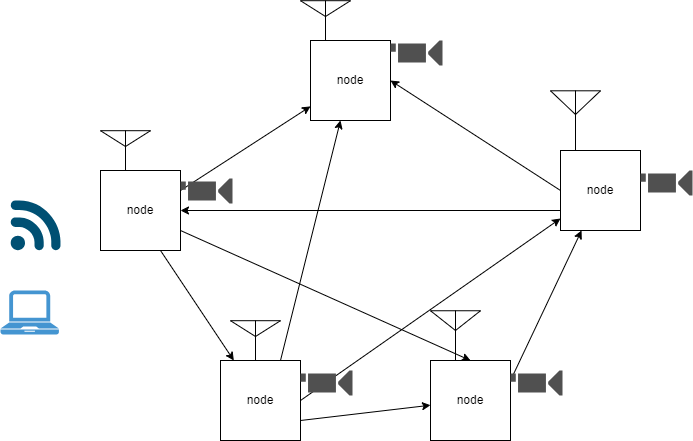
\includegraphics[width=0.5\linewidth]{Images/basic mesh network diagram.png}\par
	    \caption{Basic block diagram of a mesh network}
	
	    \label{Basic block diagram of a mesh network}
	     \end{center}
	\end{figure}

	Each node will be attached to a tree, each having a transceiver

% Body of the literature review
\section{Hardware Consideration}
In this project there needs to be data to transmit,The network needs to be able to:
\begin{enumerate}
	\item Transmit  data for  example  temperature, humidity,light and camera images.
	\item Read data every hour  and  stored it as a CSV file, The image file  will depend on the module chosen
	\item Detect  any animal that passes  the  node with a motion sensor. 
\end{enumerate}
\newpage
The following is  a  rough circuit diagram  for the project:
\begin{figure}[h!]
	\centering
	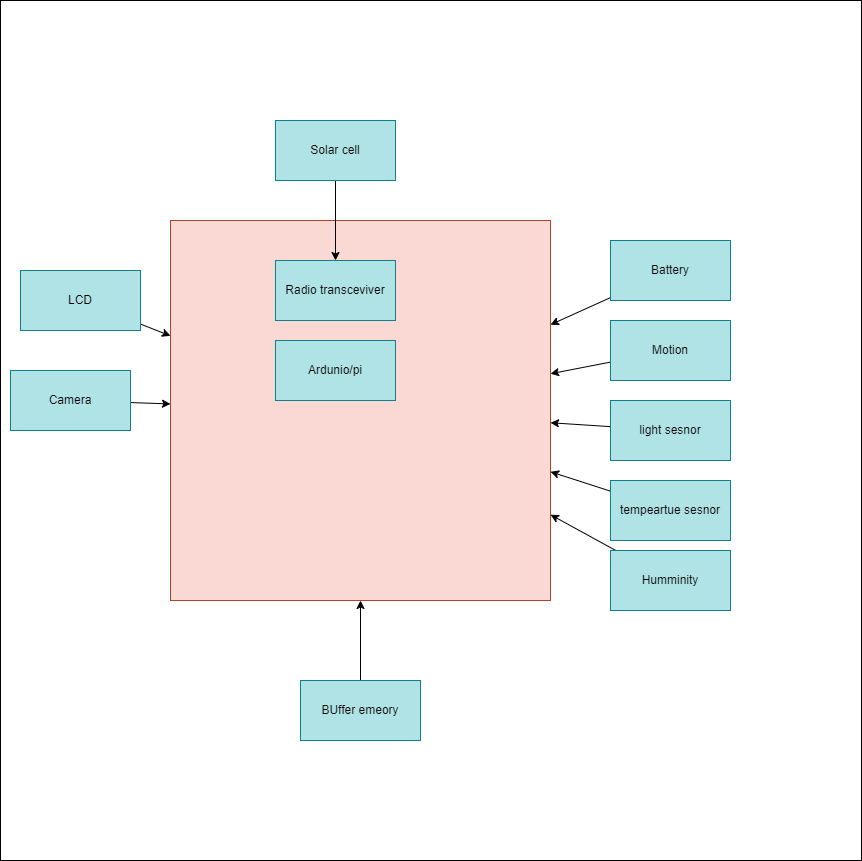
\includegraphics[width=0.5\linewidth]{Images/block_diagram_for_mesh_device.png}
	\caption{Rough circuit diagram for project}
	\label{Rough circuit diagram for project}
\end{figure}
\begin{enumerate}
	\item A PCB cannot be used due to  the ordering process taking too long for the time frame of this project 
	\item Any  type of board like wire wrap  would take too long and would be outside of  the  goals of this project
	\item A  choice of either the  Arduino or Raspberry Pi is left
\end{enumerate}
This section discusses the following:
\begin{enumerate}
	\item The sensors to be used in the project
	\item The ADC we will have  to will have to  consider
	\item The camera chosen will have to be  considered  for this project
	\item The memory module considerations
	\item The battery chosen
	\item A choice made between Arduino or Raspberry PI
\end{enumerate}

\subsection{Sensor considerations}
In this section, the process of  considering each component of the sensors will be discussed.
These components are:
\begin{enumerate}
	\item Temperature
	\item Humidity
	\item Light
	\item Motion
\end{enumerate}
\subsubsection{Temperature \& Humidity sensor}
The sensor needs to be able to work in the following conditions:
\begin{enumerate}
	\item The mesh node will be outside
	\item The device is in Ireland		\item The device is in a forest
\end{enumerate}
Taking these requirements into consideration,the temperature in Ireland was researched.

The following table was obtained from Met Eireann \cite{Eirrean}. which shows  the highest air temperature in a  shaded area
\begin{table}[h!]
	\begin{tabular}{ | c | c | c | }
		\hline
		Highest Shaded Air (°C) & Station & Date \\ \hline
		18.5°C & Dublin (Glasnevin) & 10th 1998 \\ \hline
		18.1°C & Dublin (Phoenix Park) & 23rd 1891 \\ \hline
		23.6°C & Dublin (Trinity College) & 28th 1965 \\ \hline
		25.8°C & Donegal (Glenties) & 26th 1984 \\ \hline
		28.4°C & Kerry (Ardfert Liscahane) & 31st 1997 \\ \hline
		33.3°C & Kilkenny (Kilkenny Castle) & 26th 1887 \\ \hline
		33.0°C & Dublin (Phoenix Park) & 18th 2022 \\ \hline
		31.7°C & Carlow (Oak Park) & 12th 2022 \\ \hline
		29.1°C & Kildare (Clongowes Wood College) & 1st 1906 \\ \hline
		25.2°C & Kildare (Clongowes Wood College) & 3rd 1908 \\ \hline
		20.1°C & Kerry (Dooks) & 1st 2015 \\ \hline
		18.1°C & Dublin (Peamount) & 2nd 1948 \\ \hline
		\end{tabular}
		\caption{Highest shader air Met Eireann(13$^{th}$ June 2023)}
		\label{Highest shader air Met eirrean}
	\end{table}

According to the table, the highest temperature is 33.3.The  other  extreme of the Lowest temperature was then considered:
	\begin{table}[h!]
		\begin{tabular}{ | c | c | c | }
		\hline
		Lowest Shaded Air (°C) & Station & Date \\ \hline
		-19.1°C & Sligo (Markree) & 16th 1881 \\ \hline
		-17.8°C & Longford (Mostrim) & 7th 1895 \\ \hline
		-17.2°C & Sligo (Markree) & 3rd 1947 \\ \hline
		-7.7°C & Sligo (Markree) & 15th 1892 \\ \hline
		-5.6°C & Donegal (Glenties) & 4th 1979 \\ \hline
		-3.3°C & Offaly (Clonsast) & 1st 1962 \\ \hline
		-0.3°C & Longford (Mostrim) & 8th 1889 \\ \hline
		-2.7°C & Wicklow (Rathdrum) & 30th 1964 \\ \hline
		-3.5°C & Offaly (Clonsast) & 8th 1972 \\ \hline
		-8.3°C & Sligo (Markree) & 31st 1926 \\ \hline
		-11.5°C & Wexford (Clonroche) & 29th 2010 \\ \hline
		-17.5°C & Mayo (Straide) & 25th 2010 \\ \hline
		\end{tabular}
	\caption{Lowest shader air Met Eireann(13$^{th}$ June 2023)}
	\label{Lowest shader air Met eirrean}	
	\end{table}

According to the table above the lowest temp is -19.1
In consideration for where the project the condition is a range of -19.1\textdegree C to 33.3\textdegree C.
\newpage
Humdity was also researched,Humidity refers to the amount of water vapeor in the air. The following table was obtained from Met Eireann \cite{eirrean2}:
\begin{table}[h!]
	\begin{tabular}{|c|c|c|c|c|c|c|c|c|c|c|c|c|c|}
		\hline
		\space & Jan & Feb & Mar & Apr & May & Jun & Jul & Aug & Sep & Oct & Nov & Dec & Year \\
		\hline
		Mean at 0900UTC &87.0 &86.4&84.0&79.5&76.9&76.7&78.5&81.0&83.4&85.5&88.5&88.0&83.0 \\
		Mean at 1500UTC &80.6&75.7&71.0&68.3&68.0&68.3&69.0&69.3&71.5&75.1&80.3&83.1&73.3\\
		\hline
	\end{tabular}
	\caption{Realtive Humidity(\%) according to met eirrean}
	\label{Realtive Humidity according to met eirrean}
\end{table}

The ranges are from 68.3\% to 88 \% Taking these considerations into account.Here are the different components:

\begin{table}[h!]
	\centering
	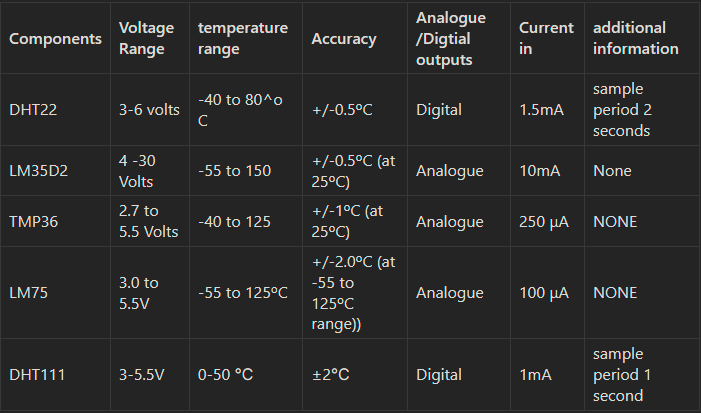
\includegraphics[width=0.5\linewidth]{Images/tempssenorscompared.png}
	\caption{Comparing of temperature sensors}
	\label{Comparing of temperature sensors}
\end{table}
After this, the choice between two sensors was narrowed down to DHT22 and DHT11. The  following are the advantages and disadvantages of the DHT22 and DHT11:
\begin{table}[h!]
	\centering
	\scalebox{0.8}{\begin{tabular}{|c|c|c|}
	\hline
		Device & Advantages & Disadvantages  \\
		\hline
		\hline
		DHT22 & good accuracy has temp and humidity, falls in our temp range & sample period 2 seconds \\
		\hline
		DHT11 & OK voltage,better sample period & draws a lot of current , and our of range \\
	\hline
	\end{tabular}}
	\caption{Comparing DHT22 and DHT11}
	\label{Compareing DHT22 and DHT11}

\end{table}

 DHT22 was chosen. Which has a  Digital output. See a wiring diagram next page:
 \newpage
This will have an interface of the following:

\begin{figure}[h!]
	\centering
	\begin{subfigure}{0.6\textwidth}
		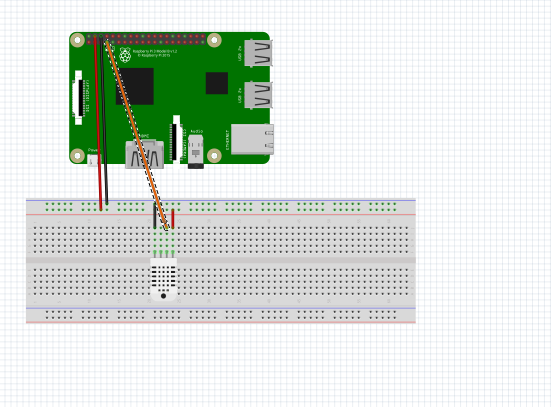
\includegraphics[width=\textwidth]{Images/InterfaceforDHT22.png}
		\caption{Interface for DHT22}
		\label{Interface for DHT22}
	\end{subfigure}
	\hfill
	\begin{subfigure}{0.6\textwidth}
		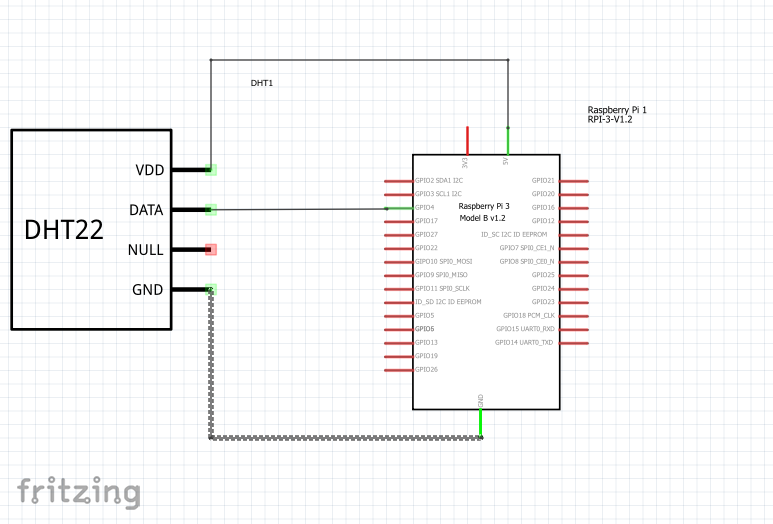
\includegraphics[width=\textwidth]{Images/schematicforDHT22.png}
		\caption{Schematic for DHT22}
		\label{Sychematic for DHT22 revised}
	\end{subfigure}
\end{figure}

From above the schematic is seen. DHT22 connections are the following:
\begin{itemize}
	\item VDD is connected to 5v of the Pi
	\item the Data pin is connected to GPIO 3
	\item Gnd pin  of the  Pi is  connected to the ground  of DHT22 

\end{itemize}
\cite{sparkfun} The following is the \href{https://www.sparkfun.com/datasheets/Sensors/Temperature/DHT22.pdf}{link} to the datasheet of this module
when reading from this  component. There is  a  delay  of 2 seconds due to the  sampling period.

\subsubsection{Light sensor}
In this section the following will be considered:
\begin{enumerate}
	\item What region the project is in 
	\item What light levels are expected in this  country
	\item What sensor  will  accommodate this  range
\end{enumerate}
\newpage
For this sensor  the outside aspect of the  project must also be considered.The following table was found on \cite{wiki_2023}:
	\begin{table}[h!]
	\centering
	\begin{tabular}{|l|l|}
	\hline
		Imminence & Example \\ \hline
		**0.002 lux** & Moonless clear night sky \\ \hline
		**0.2 lux** & Design minimum for emergency lighting (AS2293). \\ \hline
		**0.27 \& 1 lux** & Full moon on a clear night \\ \hline
		**3.4 lux** & Dark limit of civil twilight under a clear sky \\ \hline
		**50 lux** & Family living room \\ \hline
		**80 lux** & Hallway/toilet \\ \hline
		**100 lux** & Very dark overcast day \\ \hline
		**300 to 500 lux** & Sunrise or Sunset on a clear day. Well-lit office area. \\ \hline
		**1,000 lux** & Overcast day; typical TV studio lighting \\ \hline
		**10,000 to 25,000 lux** & Full daylight (not direct sun) \\ \hline
		**32,000 to 130,000 lux** & Direct sunlight \\ \hline
	\end{tabular}
	\caption{Illuminates values}
	\label{Illuminates values}
\end{table}
	This table is the  associated lux level  indicating when the values are . 
	From  above the sensor should ideally be 0.002 to 25000 lux, Bearing this in mind  these components were researched:
	\begin{table}[h!]
	\small
	\centering
	\begin{tabular}{|l|l|l|l|l|}
	\hline
		Modules & Voltage Range & Analogue /Digital Outputs & illumination range & Current rating \\ 
		\hline
		LM393 with GL5528 & 3.3v to 5v & Analogue & 0 lux to 100lux & 250nA \\ 
		\hline
		DFR0026 & 3.3v to 5v & Analogue & 1 Lux to 6000 Lux & 120uA \\ \hline
		LM393 with n5ac501085 & max 150V & Analogue & 10 lux to 100lux & 1mW \\ 
		\hline
		LM393 with NSL-06S53 & max 100v & analogue & 1 to 100 & 50mw \\ \hline
	\end{tabular}
	\caption{table of light sensors}
	\label{table of light sensors}
\end{table}
\newpage

After research DFR0026 \cite{DFR0026} is the option proposed for use as it is the best for this application,  which will have an analogue  output to see the interface (see below):

\begin{figure}[h!]
	\centering
	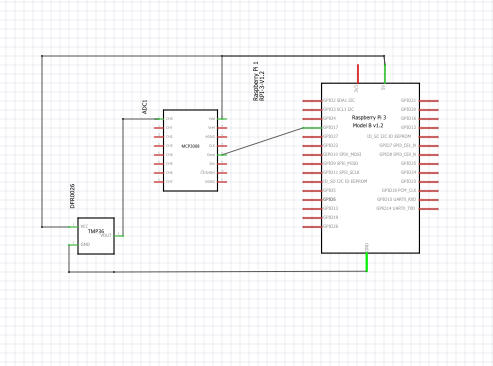
\includegraphics[width=0.6\linewidth]{Images/InterfaceofDFR0026.png}
	\caption{Interface for  DFR0026}
	\label{Interface for  DFR0026}
\end{figure}

The following are  the connections:
\begin{enumerate}
	\item VCC pin is connected  to 5v
	\item Gnd of the  sensor is connected to Gnd of the Pi
	\item The output is connected to  ch 0
	\item the output ranges  from  0 to  5 v
\end{enumerate}
The component relies on the  ADC  which  is on page\pageref{Adc section}

\subsubsection{Motion sensor}

For this section the following must be considered:
\begin{enumerate}
	\item The range of the  sensor
	\item The degree of the  sensor
	\item How long of a  delay is the sensor
\end{enumerate}
The  following are  the components considered:
\begin{table}[h!]
	\centering
	\begin{tabular}{|c|c|c|c|c|c|}
		\hline
		Modules & Voltage Range & Distance & Max angle & Analogue /Digital Outputs & Power \\
		\hline
		HC-SR501 & 5-20V & 3 to 7m & 110 & Digital & 50uA \\
		AM312 & 4.5-20v & 3m & 130 & Digital & 60uA \\
		AS312 & -0.3 - 3.6V & 12m & 130 & Digital & 100mA \\
		\hline
	\end{tabular}
	\caption{Motion sensor components}
	\label{Motion sensor components}
\end{table}

The sensor chosen is AS312\cite{micros}(which has a delay time of 2 seconds) which is a digital interface to see the wiring ,See below:
\newpage
The following is the interface for the device:

\begin{figure}[h!]
	\begin{center}
		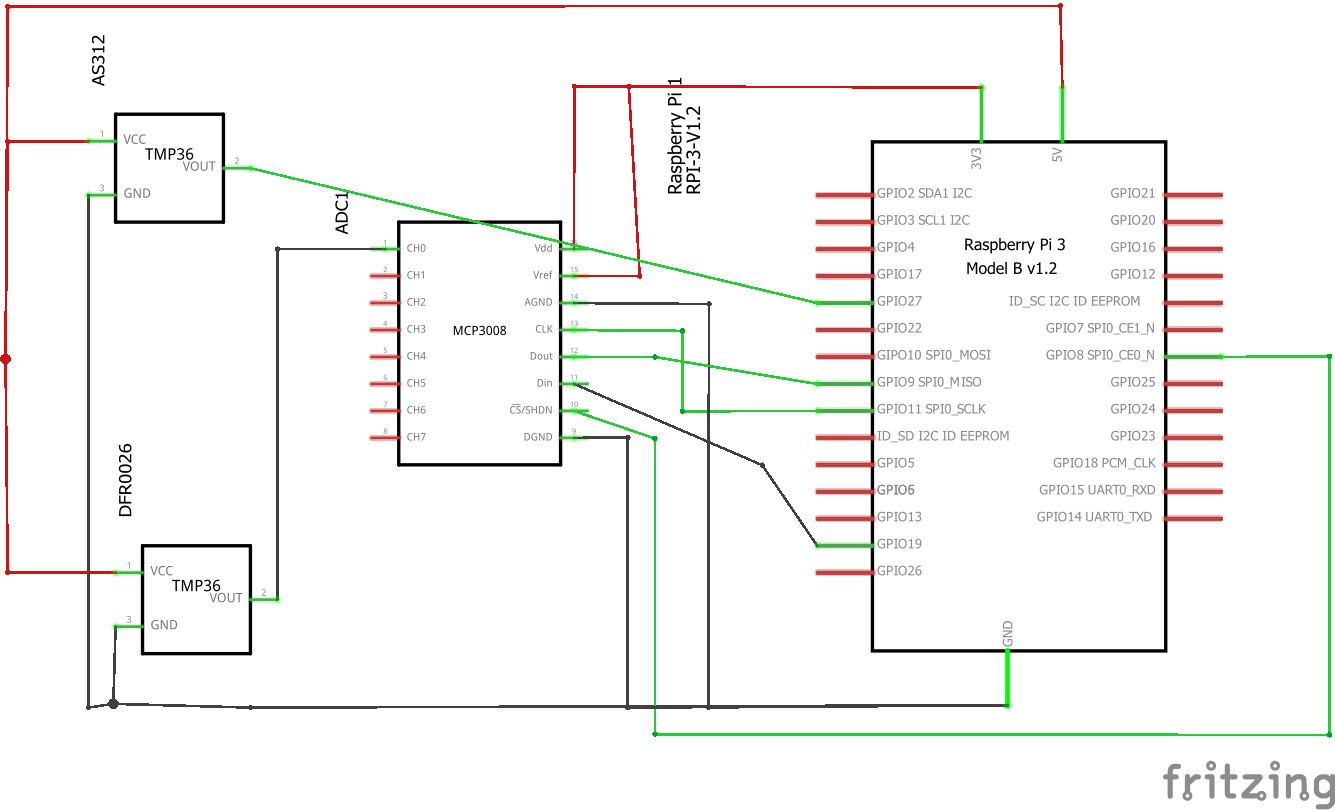
\includegraphics[width=0.5\linewidth]{Images/interfaceofAS312.png}
	\caption{Interface for AS312}
	\label{Interface for AS312}
	\end{center}

\end{figure}
The connections are the following:
\begin{figure}[h!]
	\centering
	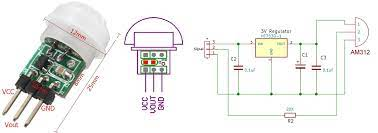
\includegraphics[width=0.5\linewidth]{Images/pinout_of_AS312.jpg}
	\caption*{Pinout of  AS312}
	\label{Pinout of  AS312}
\end{figure}
\begin{enumerate}
	\item VCC is connected  to 5v pin of the Pi
	\item GND is connected to the GND of the  Pi
	\item Vout is connected to GPIO 17
\end{enumerate}
This  component has the following:
\begin{enumerate}
	\item Range  of 12 meters 
	\item An  angle  of  65$^o$ degree
	\item A Delay of 15 $\mu$ Seconds
\end{enumerate}

\newpage
\subsection{Radio Module}
For this section there are the following considerations:
\begin{itemize}
	\item The devices are in a forest
	\item Meaning  Gigahertz  isn't  a desirable frequency
	\item A module that has low-power
	\item A model that  will have a high throughput 
\end{itemize}

Through research, I found the following table:
\begin{table}[h!]
	\centering
	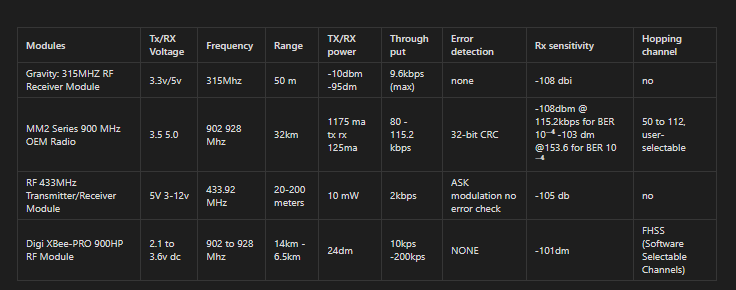
\includegraphics[width=0.5\linewidth]{Images/radiomoudles.png}
		
	\caption{Radio modules found in research}
	\label{Radio modules found in research}
	
\end{table}

Out of these, the MM2 Series 900 MHz\cite{freewave} was chosen.Note that the seller of this  radio module has  limited the documentation  of this module.This makes it hard to  draw an interface for this module .
\subsection{ADC Considerations}
\label{Adc section}
For the ADC  there are the following considerations:
\begin{enumerate}
	\item Low power
	\item High bit resolution
	\item Low number of channels
	\item High sample rate
\end{enumerate}
The two things needed for this is a high bit  Resolution  and  a  high sample rate
\begin{table}[h!]
	\begin{center}
		\begin{tabular}{|c|c|c|c|c|}
			\hline
			Device & Resolution & Sample rate & Input range & Power consumption \\
			\hline
			ADC pi Zero & 17 bits & 100KHz & 0-5.06v & 10mA \\
			MCP3008 & 10 bits & 200 ksps & 2.7v- 5.5v & 500uA \\
			DFR0553 & 16 bits & ~1.7Mhz & 0~5.0V&10mA\\
			\hline
		\end{tabular}
	\end{center}
\end{table}

Above are the components  to choose from 
for this project,MCP3008 was chosen due to its  resolution and  sample rate
\newpage
The following is the schematic for the  MCP3008\cite{ada}
\begin{figure}[h!]
	\centering
	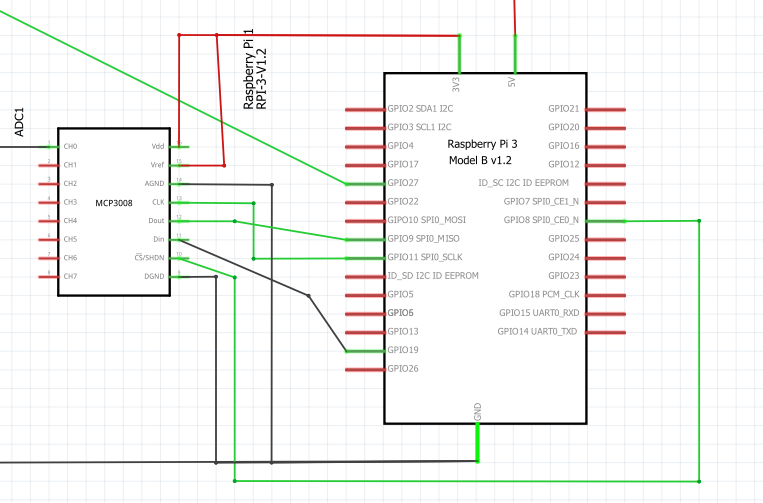
\includegraphics[width=0.6\linewidth]{Images/SchematicforMCP300.png}
	\caption{Schematic for  MCP3008}
	\label{Schematic for  MCP3008}
\end{figure}

The following are connections:
\begin{enumerate}
	\item VDD is connected to 3v3 pin of the  Pi
	\item VRef is  also connected to  3v3 pin of the  Pi
	\item AGND is connected to the gnd pin 
	\item CLK pin is connected to GPIO port 11
	\item Dout pin is connected to GPIO port 9
	\item Din pin is connected to GPIO port 19
	\item CS pin  is connected  to GPIO port 8
	\item DGND ping is connected to the gnd pin
\end{enumerate}

This  component has the following:
\begin{enumerate}
	\item A 10 bit resolution
	\item Seen as  the  reference  will  be 3.3v  
	\item 200ksps, meaning the delay to read is 5$\mu$ seconds
\end{enumerate}

\subsection{Camera}
For the camera,  the following has to be considered:
\begin{enumerate}
	\item Focal length
	\item Resolution
	\item Power
	\item The lux values it operates at
\end{enumerate}
\begin{table}[h!]
	\centering
	\scalebox{0.6}{\begin{tabular}{|c|c|c|c|c|c|c|c|c|}
	
		\hline
		Modules & Voltage range & lens size & Image Resolution & Video Resolution & Frame Rate & Type of Output & Preferred condition & Power \\
		Raspberry Pi VR 220 Camera & 3.3V ac &can change with lens & 3280 X 2462 & 1920 x 1080 &  30 FPS & Need to research & Daytime & 38mA \\
		DIGILENT 410-358 & 3.6v &  optical size 1/4 inches  & 2592 x 1944 &? &? &Digital &? & 200mA \\
		The Raspberry Pi NoIR & 3.3v  & 1/4 inches  &3280 x 2464  & 1080 or 720  &30 60 fps &need to research & house & 38mA \\
		OV7670 VGA & 2.45 to 3.0v ac & 1/6 inches & 2.36mm x 3.6um &? & 30 fps & analogue &  need to research &60mW \\
		\hline
	\end{tabular}}
	\caption{Camera module}
	\label{Camera module}
\end{table}

The camera chosen is a Raspberry Pi VR 220\cite{RS} Camera To see how to connect look at the  following \href{https://youtu.be/yhM1NhD-kGs?si=yxgFZb84yxSGLtM3}{link}. 
\subsection{Memory module}
For this section, we consider the following:
\begin{enumerate}
	\item The file formatting of the sensor data
	\item The file formatting of  the camera data
	\item What are  the possible sizes of data
	\item What is the  memory size of the  raspberry pi OS
\end{enumerate}

In my project the following is used:
\begin{enumerate}
	\item The sensor data  is stored in a  CSV file with the following heading: (timestamp, heat, humidity, light level, anything detected), Which can be around 25KB
	\item For the camera using 10 MB is the  largest file  size
	\item For the Raspberry Pi  downloaded  the raspberry imager , This has  lots of  options such as  the  following on page \pageref{pi os}
\end{enumerate}

After has been we must consider a  mircoSD ,The following are considerations:
\begin{table}[h!]
	\begin{tabular}{|c|c|c|c|c|c|c|c|c|c|}
		\hline \\
		Product Name & Capacity & Speed class & Read speed & Write speed & Temperature range & Operating volatage &Shock Resistance &Vibration Resistance \\
		\hline \hline
		SAMSUNG EVO Plus Class 10 microSDXC& 256 GB &U3&up to 130MB/s&up to 130MB/s&N/A&N/A&yes&yes \\
		SANDISK Ultra Performance Class 10 microSDXC&128 GB& class 10 u1&up to 80 MB/s&up to 10 MB/s&N/A&N/A&yes&yes \\
		Silicon Power 32GB 3D&32GB &class 10&Up to 100MB/s&Up to 100MB/s&0 to 70&2.7v - 3.6v&yes&yes \\
		SanDisk 64GB Extreme PRO&64GB&UHS Speed Class 3&Up to 100MB/s& up to 90 MB/s&N/A&N/A&yes&yes \\
		\hline
	\end{tabular}
	\caption{Mirco SDs in consideration}
	\label{mirco SDs in consirdation}
\end{table}

The best here is the silicon power 32GB due to its temperature range and read and write times.
we can consider extra memory: 
\begin{enumerate}
	\item DHTT22 has a sample period of  2 seconds
	\item AS312 which has a  delay time of 15 $\mu$ seconds
	\item MCP3008 5 $\mu$ seconds
\end{enumerate}

Through research,the following was discovered :
\begin{table}[h!]
	\centering
	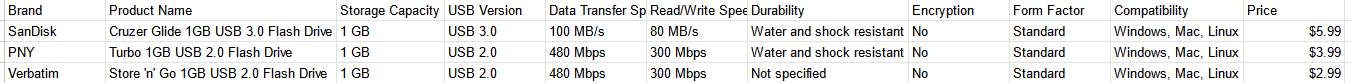
\includegraphics[width=0.8\linewidth]{Images/memory_devices.png}
	\caption{Memory usb to consider}
	\label{Memory usb to consider}
\end{table}

The Raspberry Pi 4 supports USB 2 and  USB 3. For this, the Turbo 1GB USB 2 Flash Drive will  be chosen.

\subsection{Battery}
In this section the  following must be considered:
\begin{enumerate}
	\item Enough power for all  sensors  and  radio module
	\item Storage of the battery
	\item Discharge rate of the  battery (how many operating hours can be got out of the  battery)
\end{enumerate}
Here are the following  Devices I found :
\begin{table}[h!]
	\centering
	\begin{tabular}{|c|c|c|c|c|c|}
		\hline
		Modules & Voltage & Interface & Power & Chemistry & Supply time\\
		\hline
			Li-polymer Battery HAT  & 5v & Micro USB & 1.8A &lithium battery &5 hours \\ \hline
	\end{tabular}
	\caption{battery considerations}
	\label{battery considerations}
\end{table}

The battery chosen  is the li-polymer which has a micro USB 
How to charge:
\begin{itemize}
	\item Step 1: Insert the Li-polymer battery into a 2.0mm battery socket
	\item Step 2: Connect the power adapter to a micro USB or Type-C interface by USB cable.
\end{itemize}

Aside: this component has the following:
\begin{enumerate}
	\item A battery that is 3.7v 3000$mAh$ 
	\item Output voltage of 5 volts
	\item an estimated Power supply time  of  5 hours
\end{enumerate}
\subsection{Arduino vs PI Consideration }
In this project, we will have to choose between what microprocessor we will use.There are 3 options:
\begin{enumerate}
	\item PCB (printed circuit board)
	where the circuit is deigned in a program like Fusion 360. The major issue is due to  the current state of  silicon chips which will slow down  the progress of the implementation stage
	\item Arduino 
	\item Raspberry Pi
\end{enumerate}

The advantages and disadvantages of the Arduino and  the Raspberry Pi are the following:
\begin{table}[h!]
	\centering
	\begin{tabular}{|c|c|}
		\hline
		Arduino & Pi \\
	
	\hline \hline
	Advantages & Advantages \\
	\hline \hline
	1. Arduino has a 10-bit ADC & 1. Pi can compile Python (easier to write ) \\

	\hline \hline
	Disadvantages & Disadvantages \\
	\hline \hline
	1. Arduino has a supper set of C++ & 1. Pi is a technically a small CPU \\
	2. Arduino only has 6 Analogue pins  & 2. The Pi needs an ADC circuit to deal with inputs that are analogue \\
	
	\hline
	\end{tabular}
	\caption{Advantages /Disadvantages of Arduino vs pi}
	\label{Advantages /Disadvantages of Arduino vs pi}
\end{table}

Although the  Arduino would be more efficient than the Raspberry Pi due to Raspberry Pi has an Operating System . The Pi was picked due familiar with Python and Linux. Linux can  be used to handle the networking side  of   the project
At the cost of  some efficiency in power for an easier time writing the code for  this  project 
\subsubsection{Picking a Raspberry Pi}
Now that a device was chosen to  use the following need to be defined:
\begin{enumerate}
	\item The amount of GIPO PORTS we need 
	\item Nature of the output of the sensor
	\item Speed of the clock
\end{enumerate}	

GPIO(General purpose input/output) is used  to select the input/output. The Pi can  take in  digital signals only Seen as the components are chosen that require A GPIO port (temperature/ humidity, on page \pageref{Compareing DHT22 and DHT11}, Light on page \pageref{table of light sensors}, motion on page \pageref{Motion sensor components})

At least  3 GPIO ports to be available to us as the light sensor and the motion will  need  an adc as looking through the documentation .firstly let's look at the  different models:
\begin{table}[h!]
\scalebox{0.6}{\begin{tabular}{|l|l|r|l|l|l|1|}
	\hline
	\rowcolor[HTML]{CE6301} 
	Raspberry Pi Model      & Internal Clock Speed & \multicolumn{1}{l|}{\cellcolor[HTML]{CE6301}Power (Watts)} & GPIO Features & Type of Connectors                                                            & SRAM                   \\ \hline
	Raspberry Pi 1 Model B+ & 700 MHz              & 5.5                                                        & 26 GPIO pins  & 1 HDMI, 1 micro USB, 1 USB 2.0, 1 audio jack                                   & 512 MB                 \\
	Raspberry Pi 2 Model B  & 900 MHz              & 7.5                                                        & 40 GPIO pins  & 1 HDMI, 1 micro USB, 4 USB 2.0, 1 audio jack                                   & 1 GB                   \\
	Raspberry Pi 3 Model B+ & 1.4 GHz              & 8                                                          & 40 GPIO pins  & 1 HDMI, 1 micro USB, 4 USB 2.0, 1 audio jack, 1 Gigabit Ethernet, 1 PoE header & 1 GB                   \\
	Raspberry Pi 3 Model A+ & 1.4 GHz              & 5                                                          & 26 GPIO pins  & 1 HDMI, 1 micro USB, 2 USB 2.0, 1 audio jack                                   & 512 MB                 \\
	Raspberry Pi Zero       & 1 GHz                & 1.2                                                        & 40 GPIO pins  & 1 mini HDMI, 1 micro USB, 1 micro-USB OTG                                      & 512 MB                 \\
	Raspberry Pi Zero W     & 1 GHz                & 1.3                                                        & 40 GPIO pins  & 1 mini HDMI, 1 micro USB, 1 micro-USB OTG, 1 Wi-Fi/Bluetooth module            & 512 MB                 \\
	Raspberry Pi Zero 2 W   & 1 GHz                & 0.8                                                        & 40 GPIO pins  & 1 mini HDMI, 1 micro USB, 1 micro-USB OTG, 1 Wi-Fi/Bluetooth module            & 512 MB                 \\
	Raspberry Pi 4 Model B  & 1.5 GHz              & 7                                                          & 40 GPIO pins  & 2 HDMI, 2 USB 3.0, 2 USB 2.0, 1 Gigabit Ethernet, 1 audio jack                & 1 GB, 2 GB, 4 GB, 8 GB \\ \hline
	\hline
\end{tabular}
}
\caption{Table of Raspberry Pi's}
\label{Table of Raspberry Pi's}
\end{table}

The above table displays the modules ,As our radio modules is 900Mhz  we want  1.5GHZ which is the Raspberry Pi 4.This needs a USB\- c charger and an HDMI mini cable.
For wiring our Pi here is  the GPIO pin layout:
\begin{figure}[h!]
	\centering
	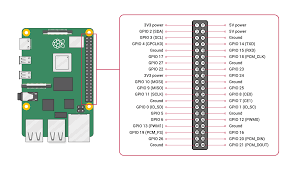
\includegraphics[width=0.8\linewidth]{Images/Pinout_of_pi.png}
	\caption*{Pinout for  the  pi}
	\label{Pinout for  the  pi}
\end{figure}

\subsection{Conclusion}
In this project the hardware needed is the  following components:
\begin{enumerate}
	\item 1 x Raspberry Pi 4 Model B 
	\item 1 x HDMI cable
	\item 1 x USB\-C cable
	\item 1 x USB \-C charging head
	\item 1 x DHT22
	\item 1 x DFR0026
	\item 1 x AS312
	\item 1 x MM2 Series 900 MHz
	\item 1 x MCP3008
	\item 1 x Raspberry Pi VR 220 Camera
	\item  1 x Li-polymer Battery HAT 
	\item 1 x Turbo 1GB
	\item 1 x silicon power 32GB  microSD
	
	
\end{enumerate}
\section{Software considerations}
Having established the essential hardware needed for this project. Next, consider the following  for the software of the  project:
	\begin{enumerate}
	    \item How to structure code 
	    \item Linux set up of sever and nodes
	    \item How will data be sent
	    \item Will this be an OOP or functional approach?
	    \item How to program each device?
	\end{enumerate}
	\subsection{Raspberry Pi OS}
	\label{pi os}
	In this section, it must be kept in mind  that each OS is  heavyweight the following needs to be considered:
	\begin{enumerate}
		\item If the SD is formatted the data on the SD is lost. Does it corrupt the card?
		\item An os that is low in capacity 
		\item Is a desktop needed or can we use the terminal?
		\item How does the OS  respond to USB drives?
	\end{enumerate}

	According to the \cite{projects} the imager will erase all the data while installing the os. From research, the suggestion of backing up the data is a good suggestion.
	for now, the recommended OS is used. and strip down as the project progresses. which will be discussed in the methodology section of this report.
	
	\subsection{Sensor code}
	In this section, the following will be discussed :
	\begin{enumerate}
		\item DHT22
		\item AS312
		\item MCP3008
		\item DFR0026
		\item Kuman for Raspberry Pi 3B+ TFT LCD Display
		\item Raspberry Pi VR 220 Camera 
	\end{enumerate}

	the project code will mainly be object-oriented. so the goal is to first test it with my laptop and  Create A bash file full of commands to install the libraries, making the code split up into different parts so that all that is needed is the libraries used and code that won't all have to be compiled in one file.

	\subsubsection{DHT22}
	In this section we have to consider the following: 
	\begin{enumerate}
		\item The GPIO port as on page \pageref{Sychematic for DHT22 revised} This is connected to port 3 
		\item The type of output is digital so no  extra hardware/code is needed
	\end{enumerate}

	The following is a rough guide on how to read from the DHT22 from the following \href{https://www.instructables.com/Raspberry-Pi-Tutorial-How-to-Use-the-DHT-22/}{link}.
	Firstly open the terminal in the Pi and
	type the following commands:
	\begin{lstlisting}[style=bashstyle]
		git clone https://github.com/adafruit/Adafruit_Python_DHT.git
		cd Adafruit_Python_DHT
		sudo apt-get update
		sudo apt-get install build-essential python-dev
		sudo python setup.py install
	\end{lstlisting}
	the code does the following:
	\begin{enumerate}
		\item firstly git clone will clone the  repository onto to device
		\item Then change directories  a
		\item update Linux
		\item install dev kit for  python 
		\item and install the setup 
	\end{enumerate}
	
	this will then lead to  the  following code:
	\begin{lstlisting}[style=mystyle,caption={Example code for DHT2},numbers=left,firstnumber=1]
		#Libraries
		import Adafruit_DHT as DHT
		from time import sleep
		def setup_DHT22(Gpoiport:int):
		humidity,temp=dht.read_retry(DHT.DHT22, Gpoiport)
			sleep(5)
			return humidity, temp
		h,t=setup_DHT22(3)
		print('Temp={0:0.1f}*C  Humidity={1:0.1f}%'.format(t,h))
	\end{lstlisting}
	this code will do the following:
	\begin{enumerate}
		\item Import DHT from the Adafuit library
		\item in the  function which takes the GPIO port  as an integer this will read the data on the pin and  print it  out
	\end{enumerate}
	
	\subsubsection{AS312}
	for this section i followed  this \href{https://pimylifeup.com/raspberry-pi-motion-sensor/}{link}
	we also want to keep in mind the following:
	\begin{enumerate}
		\item This has a  digital interface and is connected  to GPIO 27 
	\end{enumerate}
	Here are the rough steps firstly  type the following into the  terminal 
	\begin{verbatim}
		sudo apt-get install python-rpi.gpio
	\end{verbatim}
	which will install a gpio python module
	Then type this into an IDE of your  choosing
	\begin{lstlisting}[style=mystyle,caption={Example code for AS312},numbers=left,firstnumber=1]
		import RPi.GPIO as GPIO
		import time

		pir_sensor = 27
		GPIO.setmode(GPIO.BOARD)

		GPIO.setup(pir_sensor, GPIO.IN)
		current_state = 0
		
		time.sleep(0.1)
		current_state = GPIO.input(pir_sensor)
		if current_state == 1:
			print("GPIO pin %s is %s" % (pir_sensor, current_state))
			# trigger camera
		# must look up this 
		GPIO.cleanup()
	\end{lstlisting}
	this code does the  following:
	\begin{enumerate}
		\item it will look at the  pin for a pulse 
		\item Once it senses a pulse  it will trigger  the camera
	\end{enumerate}
	\subsubsection{DFR0026}	
	from the last example, nothing has changed from the last component
	an example code for this can be found on page \pageref{adc code}
	\subsection{MCP3008}
	for this section, we want to consider the following:
	\begin{enumerate}
		\item The MCP3008 data out is GIPO 9 
	\end{enumerate}
	This section follows this \href{https://randomnerdtutorials.com/raspberry-pi-analog-inputs-python-mcp3008/}{link}
	firstly try the following in command in the terminal 
	\begin{verbatim}
	sudo raspi-config nonint do_spi 0
	\end{verbatim}
	
	\label{adc code}
	\begin{lstlisting}[style=mystyle,caption={ADC code},numbers=left,firstnumber=1]
		from gpiozero import MCP3008
		from time import sleep
		DFR0026 = MCP3008(channel=0, device=0,port=9)
	
		print ('raw: {:.5f}'.format(DFR0026.value))
		sleep(0.1)
	\end{lstlisting}
	this code will select a  channel and device, port and  print the values of the ADC's
	\subsection{Raspberry Pi VR 220 Camera}
	to get started with this simply look at the following \href{https://projects.raspberrypi.org/en/projects/getting-started-with-picamera/4}{link}
	here is an example of the code of this module :
	\begin{lstlisting}[style=mystyle,caption={example code for camera},numbers=left,firstnumber=1]
		from picamera import PiCamera
		from time import sleep

		camera = PiCamera()

		camera.start_preview()
		sleep(5)
		camera.stop_preview()
	\end{lstlisting}
	this will  take a photo of what is in front of the  camera

	\subsection{MM2 Series 900 MHz}
	for this section, the seller of this module has no public  documentation so it is hard to  come up with  an make interface for  this section   
	\subsection{code structure}
	The code structure for this  will be an object-oriented program all the individual sensors and  hardware  for the pi will be as displayed above the code in this section will be formatted into objects for example I will have an  object   called proj\_sensor and  a method of this  would be  DHT22 while an attribute of this would  be  the  sample rate
	the following is a  rough breakdown of the  structure of the code
	\begin{itemize}
		\item Sensor object
		
		\begin{itemize}
			\item Temperature and humanity method
			\item light method
			\item Motion method which triggers the camera
			\item Battery method which is a constructor method
			\item Memory method which  links with the radio 
		
		\end{itemize}
		
		\item radio object which reads from Memory and  transmits the data 
	
	\end{itemize}
	\subsection{File structure}
	For the  File structure, we want our sensor data to be stored every hour in a  CSV file with the following column headings:
	\begin{enumerate}
		\item timestamp
		\item Heat
		\item Humidity
		\item light level
		\item motion detected (True/False)
	\end{enumerate}
	for the writing to Date, we will use Pandas to write to the CSV file
	for file sorting, I will use the Python Library glob  which I can use  to look for  files 
	the following is an example of how  to  make a CSV file:
	firstly let's make a data frame:
	\begin{lstlisting}[style=mystyle,caption={sample code for turning sensor data into a data},numbers=left,firstnumber=1]
		import pandas as PD
		import numpy as np
		from datetime import datetime
		cols_name=["Timestamp", "Temperature", "Hummidty", "Light_level", "Motion_dected"]

		#assume that being recorded now
		data=[]
		timestap=datetime.now()
		timestap=timestap.strftime("%d/%m/%Y %H:%M:%S")
		Current_state=1
		Heat=0.40
		Hummidty=1.0
		Light_level=0.23
		data=np.array([[timestap],[Heat],[Hummidty],[Light_level],[Current_state]])
		data=data.T
		df= pd.DataFrame(data,columns=cols_name)
	\end{lstlisting}
	Next, use the.To\_csv method from  pandas
	another Libraries that could  be useful is the Tkinter
	here is a  sample of how to   store where the  file is  gonna be:
	\begin{lstlisting}[style=mystyle,caption={example code for storing directory},numbers=left,firstnumber=1]
		import tkinter as tk
		from Tkinter import filedialog
		import json
		import os

		root = tk.Tk()
		root.withdraw()
		selected_dir = filedialog.askdirectory()

		if not os. path.exists('selected_dir.json'):
			# Write the selected directory to a JSON file
			with open('selected_dir.json', 'w') as f:
				json.dump(selected_dir, f)
				print("Successfully saved selected directory to JSON file.")
		else:
			print("File 'selected_dir.json' already exists. Not saving the directory.")

		root.quit()
	\end{lstlisting}
	Other useful Libraries allow you to  select all  .csv, png  called glob
	for our TDD Section, we will have to use the  following command:
	\label{TDD sample bash}
	\newpage
	\begin{verbatim}
		# !/bin/bash

		dir_name=$1

		size=$(du -sh "$dir_name" | cut -f1)

		echo "Directory size: $size"
	\end{verbatim}
	This is a script that will look at a  director this can be a home directory that will call the  space 13K
	the "| cut -f1" will only focus on the size string message and then print out the size. this is  just  a sample  script 
	\subsection{Test Driven development}
	In this  project ill will be using  Test Driven Development (TDD) is a software development approach where tests are written before the actual code
	the following are the advantages of TDD:
	\begin{enumerate}
		\item Advantages
		\begin{enumerate}
			\item TDD forces you to consider potential failure points and edge cases upfront, leading to earlier detection and resolution of bugs.
			\item TDD encourages you to think about the desired behavior and interfaces of your code
			\item TDD provides immediate feedback on whether your code works as intended,
		\end{enumerate}
	\end{enumerate}

\section{Attenuation}

Attenuation refers to a reduction in the strength of a signal.
 Attenuation occurs with any signal, whether digital or analogue. 
Seen the aim of making a network the first step is to look into  
what frequencies can be transmitted and received.
\newline
In the environment in which we want our project to take place, we want the following:
 \begin{enumerate}
	\item An antenna that a high so we can affect the data rate of the signal
	\item A frequency range at which Attenuation is not present 
 \end{enumerate}
Through research, I found the following plots:

\newpage

\begin{enumerate}

	\item  First Plot
	The first plot  I got for Savage e.t al pg. 7 \cite{Savage}
	\begin{figure}[h!]
		\centering
		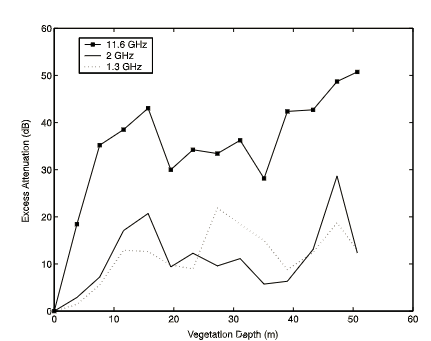
\includegraphics[width=0.5\linewidth]{Images/Silver_Maple.png}
		\caption{Silver Maple in-leaf excess attenuation for the line of trees geometry (receiver antenna height: 3.5 m, SAVAGE ET AL.pg.7}
		\label{Silver Maple in-leaf excess attenuation for the line of trees geometry (receiver antenna height: 3.5 m, SAVAGE ET AL.pg.7}
	\end{figure}
 
This graph displays as vegetation depth increases  Attenuation rises. The problem with this graph is that it doesn't give an in-depth view of which attenuation occurs.
This then led me to look up the International Telecommunication Union  \cite{ITU} recommendations for Attenuation in wooded areas



	\item Second Plot
\begin{figure}[h!]
		\centering
		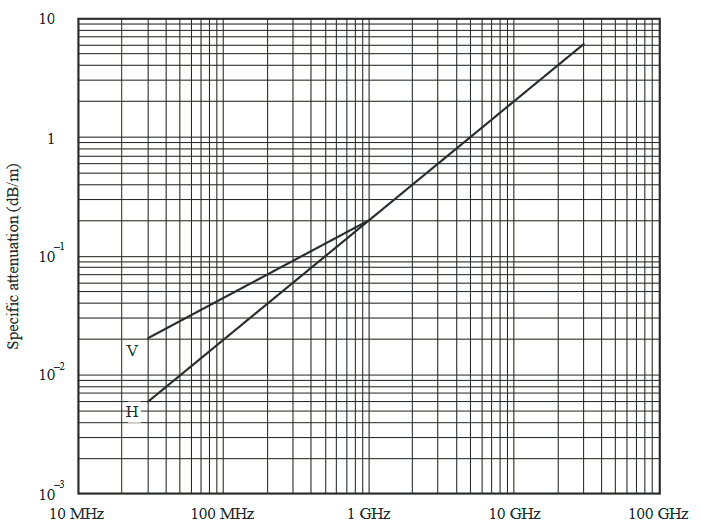
\includegraphics[width=0.5\linewidth]{Images/ITU attteuntion.png}
		\caption{Specific attenuation due to woodland (Recommendation ITU-R P.833-7 (02/2012) Attenuation in vegetation pg.5}
		\label{Specific attenuation due to woodland (Recommendation ITU-R P.833-7 (02/2012) Attenuation in vegetation pg.5}
		\end{figure}
	V is the vertical polarization
	H is the horizontal polarization

	From this graph we  can assume the following:
	\begin{enumerate}
		\item From a frequency $\ge$15GHz we can assume Attenuation is more components
		\item Around the 1 GHz range we  get low values of Attenuation
		\item in the  MHz range we get the best response
	\end{enumerate}
	from this, I selected the  range which is  $10^6 hz$
	
\end{enumerate}
\newpage
so now that  we  established our range let us consider  what happens when it rains\cite{Sabetahd_Mousavi_Ghasemi_Vafaei_Poursorkhabi_Mohammadzadeh_Zandi_2022}

\begin{figure}[h!]
	\begin{center}
		
	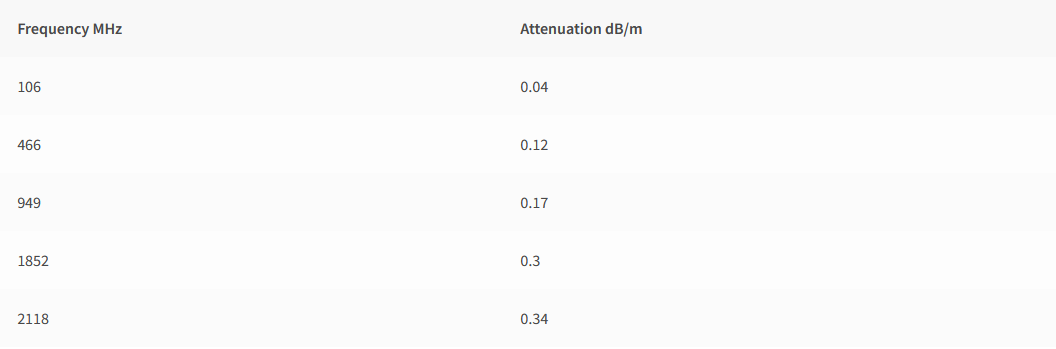
\includegraphics[width=\linewidth]{Images/atteuntion_2.png}\par
	\caption{Predicted attenuation due to rain for the region, which is measured by using the ITU standards,(Source: Hindawi(2014))}
	\label{Predicted attenuation due to rain for the region, which is measured by using the ITU standards,(source: Hindawi(2014))}
		\end{center}
\end{figure}
Ideally, we want a low MHz but we want speed and this  is dictated by what we choose let's further see how radio waves are affected by water/rain
\subsection{Absorption of water}
for this, I found this graph from Lunken Heimer \cite{lunken} 

\begin{figure}[h!]
	\centering
	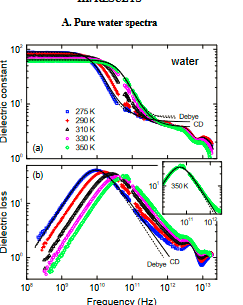
\includegraphics[width=0.5\linewidth]{Images/absorstion.png}
	\caption{absorption of water}
	\label{absorption of water}
\end{figure}

According to the  graph, Water absorbs MHz frequencies which will affect the  transmission 
in the transmission and in some cases, we might have to consider non-line-of-sight communication when it rains or we might also consider another node to route to receive the node.





\section{mesh network considerations}
For this section, we have to consider the following:
	\begin{enumerate}
		\item How are we setting up the network
		\item What framework are we using to set this Up
		\item What are the advantages/disadvantages
	\end{enumerate}
	In my research I found two main frameworks that this project could use to achieve the mesh network these are the following:
	\begin{enumerate}
		\item LORA
		\item Zigbee
	\end{enumerate}
	According to Chen (2023)\cite{chen} "LoRa, as one of Low Power Wide Area Networks (LP-WANs) technologies, aims to enable IoT devices to perform long-range communications with lower power consumption [18]. LoRa makes use of the chirp spread spectrum (CSS) modulation to improve the transmission distance up to kilometres and also be resistant to multi-path effects."
	\par
	According to Vlad\cite{Gavra_Pop_Dobra_2023}, "ZigBee is an LP-WPAN (Low-Power-Wireless Personal Area Network) with short range and low power consumption, as mentioned before. The range for ZigBee devices is up to fifty meters and it is characterized by a low data rate, having a maximum value of 250 kbps. The protocol is suitable for sensors and IoT applications because of the low data rate and low power consumption"
	\par
	the following are the  differences between the two:
	\begin{table}[h]
		\centering
		
		\begin{tabular}{|c|c|c|c|}
		\hline
		\multicolumn{2}{|c|}{LoRa} & \multicolumn{2}{|c|}{ZigBee} \\
		\hline
		Advantages & Disadvantages & Advantages & Disadvantages \\
		\hline
		Long transmission distance & Low transmission rate & Low power consumption & Low data rate \\
		Low power consumption & Slow data transfer rate & Long range & Limited range \\
		Multi-channel information procession & Small payload & Scalability & Signal interference \\
		Strong anti-interface ability & Low bandwidth & $-$ & High-sensitivity levels \\
		High-sensitivity levels & Spectrum interference \\
		\hline
		\end{tabular}
		\caption{Advantages and Disadvantages of LoRa and ZigBee}
		\label{tab:lora_zigbee}
		\end{table}
		from research, these are very  similar  but it seems if I plan on adding lots of Zigbee is the best for this challenge  

\section{Review  key of research Papers}
The following are the research papers I used
\begin{enumerate}
	
	\item zhao
	
		In my research, I found  multiple projects that are similar to mine 
		In Zhao(2023)\cite[zhao]{zhao}  
		used  LORA to  track  light sensitivity, air pressure
		one of the challenges Zhao came across was Attenuation as stated above and also the author came across the problem of not having sufficient solar panels 
	\item Daniel
	
		Another paper I found in my research is by Daniel \cite{Daniel}
		In this, Daniel discusses modeling radio wave propagation in a forest environment which isn't in the scope of the project
		Daniel's work shows that a better approximation  for transmission loss was a key read to  under what happens on a more in-depth scale in my project
	
	\item Anna
	
		\cite{Anna} in Anna's paper  she  mainly used LORA where she compared line of sight and  the  non-line  line of sight environments in  urban and  forested areas
		this paper aims to study the effects of signal propagation in different environments.
	

	\item ITU
	
		\cite{ITU} in ITU in most research papers I found  it  referred back to this  document this document was  very helpful in terms  of  understanding Attenuation  and challenges that face

\end{enumerate}


\section{Summary}
This report  highlights the  challenges at come from  transmitting data in a  wooded area these challenges are  the following:
\begin{enumerate}
\item Attenuation 
\item Absorption
\end{enumerate}
In a wooded area, we established that  Attenuation occurs due to the reflection, and penetration of radio through any type of medium.
We established that our antenna will have to  be in the  Mhz range   but will still have signal loss /errors due to Absorption of  the  signal  received due  to rain or water being in the signal path
we have yet to consider the non-line of sight environment but this  is  to be  discussed when prototyping, this report mainly focuses on the hardware where the  focus is on  sensors such as:
\begin{itemize}
\item Temperature
\item Light
\item Motion
\item Humidity
\end{itemize} 
The report focuses on how to read this data from a  Software perspective the code will be an object-oriented program
where the code will be separated into different blocks of code so the file size is minimized and leads to a faster compile time. 




\chapter{Methodology}
\section{Methodology}
\subsection{Introduction}
In this  Section  i will discuss the  proposed  methodology of this  project this will cover the  following:
\begin{enumerate}
    \item The Research Philosophy
    \item The Research Approach
    \item The Research Design
    \item The Data Collection Methods
    \item The Model Development
    \item The Data Analysis Methods
    \item The Ethical Considerations
    \item The validity and reliability 
    \item The Limitations and Delimitation
    \item The timeline
\end{enumerate} 
\subsection{Research Philosophy}

This research adopts a pragmatic philosophy, which emphasizes the practical application of knowledge and the need for researchers to be flexible and adaptable in their approaches. This aligns well with the computational nature of the research, as it allows for the exploration of different methods and techniques to achieve the research goals.

\subsection{Research Approach}

This study employs a computational research approach, which involves the development and utilization of software tools and algorithms to address research questions. Computational methods are well-suited for handling large datasets, complex systems, and experimental simulations.

\subsection{Research Design}

\subsection{Data Collection Methods}
In this section  i dicuss the  following:
\begin{enumerate}
    \item the  intall  unit test this is for  what we  expect  our  sensor  to  output this  will  be  updated
    \item How  the data  from sensor will be stored 
    \item the code  assoicated   with the above points 
\end{enumerate}
\subsubsection{Unit testing}
Fristly i want to made  some unit tests the aim of this  is the  following:
\begin{itemize}
    \item To make  test  that will be  there for  the  codeing  section of  the  project 
\end{itemize}
this section will discuss the  following for  testing:
\begin{enumerate}
    \item 1 x DHT22
    \item 1 x DFR0026
    \item 1 x AS312
    \item 1 x MM2 Series 900 MHz
    \item 1 x MCP3008
    \item 1 x Raspberry Pi VR 220 Camera
    \item  1 x Li-polymer Battery HAT 
    \item 1 x Turbo 1GB 
\end{enumerate}
\subsubsection{DHT22}
According to the  data sheet \cite{sparkfun} seen as  the data is   8 bits  and  the  range at which this   operates at  -40 to 80$^{o}$c for tempeature
meaning we have  at least  7 bit in the  exponent to  represent  the   measured value.
to represent  the  high  end of this  sensor i used the  following calculation:
$$ 2^6 +2^4 = 80$$ which mean  we have  a 2 bits dedicated to decimal place so the  high temperature to be 80.3$^{o}$c
for the  lowest temp we have 6 bits  to  represent  - 40 due to  2s complement  so lowest  will   be -40.3$^{o}C$
so with that  that  stablish we  must  make a  unit  that will do  the  following:
\begin{enumerate}
    \item Test if the  output is  a float
    \item Test the  high end of  the  temp sensor so it  reads  80.3 as  the highest
    \item Test for the  lowest   temp   around 
\end{enumerate}
be sure to follow  steps  for  folder  setup  follow instructions on page \pageref{folderstructure}.
we get the following sample code:
\begin{lstlisting}[style=mystyle,caption={sample test intial code}]
import unittest
from protest import Read_DHT22
class test_project_code(unittest.TestCase):
    def test_DHT_22_temp_output_type(self):
        self.assertIsInstance(Read_DHT22, float)
    def test_DHT22_temp_range(self):
        self.assertGreaterEqual(Read_DHT22,-30.3)
        self.assertLessEqual(Read_DHT22,80.3)
    
\end{lstlisting} 
This code import unitest . the from protest is  a python files  we can  install  functions from other python files this can be usefull for testing purposes
then we initalized a test class call Unittest.testcase our firstion fucntion of the class  we  check if the number of the output  is a float or not this is  for  testing  tempearture
the next function we test for  is the range i look at the datasheet online   this code is  simpley testing the  limits of the  DHT22
for  humidity  the Datasheet which ranges from 0 to 100 \%
we want to test for the following:
\begin{enumerate}
    \item Test if the  output is  a float
    \item Test if the  output ranges 0 to 100
\end{enumerate}
this lead to the  following code 
\begin{lstlisting}[style=mystyle,caption={sample test for DHT22}]
import unittest
from protest import Read_DHT22
class test_project_code(unittest.TestCase):
    hum,temp=Read_DHT22(2)
    def test_DHT22_output_type(self):
        self.assertIsInstance(Read_DHT22,tuple)
    #....

    def test_DHT22_hum_output_type(self):
        self.assertIsInstance(hum,float)

    def test_DHT22_hum_range(self):
        self.assertGreaterEqual(hum,0.0)
        self.assertLessEqual(hum,100.0)
\end{lstlisting}
seen as we expect our sensor to  print out a humdity and temp values we  set the  output to  a tuple 
to test for this we use isInstacne which will test if its a tuple
next we test for the  limits of the  humidity
\subsubsection{DFR0026 \& MCP3008}
According to the  datasheet \cite{ada} we must keep in mind  that this  componet is  connected to  an ADC 
this  will  give  me  the  following  test conditions:
\begin{enumerate}
    \item Test if  the output is a float

    \item Test  the  range of this  with the  upper limit being 5v 
    \item test the  lover limit being 0 
\end{enumerate}
\begin{lstlisting}[style=mystyle,caption={unit test for  DFR0026 and  MCP3008}]
    import unittest
    from protest import Read_DHT22,Read_MCP3008
    class test_project_code(unittest.TestCase):
    def test_DFR0026_MCP3008_out_type(self):
        self.assertIsInstance(Read_MCP3008,float)
    def test_DFR0026_MCP3008_out_range(self):
        self.assertLessEqual(5.0000000)
        self.assertGreaterEqual(0.0000000)
\end{lstlisting}
this code is in the same in theres of limits
\subsubsection{AS312}
for  this section  we  want our  tests  to  be  the following:
\begin{enumerate}
    \item test for type is boolean 
\end{enumerate}
we can  now add to the snipppet :
\begin{lstlisting}[style=mystyle,caption={unit test for AS312}]
    def test_AS312_out_type(self):
        self.assertIsInstance(Read_AS312,bool)
\end{lstlisting}
\textbf{Note : Don't forget to import read_as12 function from test file}
seen as  thhis is a motion sensor  our ouout will be true or false
\subsubsection{Raspberry Pi VR 220 Camera}
according to the  data sheet \cite{Camera}
we the  resoultion to  it uses is  1080p50 which is 1920x1080p so our  tests will have to  in copoarte  the  followoing:
\begin{enumerate}
    \item Test the  output shape  if open cv is  gonna  be  used 
    \begin{enumerate}
        \item test  the  amout of   elelecelm in the  3 dimesional   array 
    \end{enumerate}
    \item test the  file  type  is png
\end{enumerate}
this would lead me to the following code snippet.
\begin{lstlisting}[style=mystyle,caption={camera unit test}]
    def test_Raspberry_Pi_VR220_out_shape(self):
    self.assertEqual(Read_Raspberry_PiVR220.shape,(1920,1080,3))
\end{lstlisting}
this function check the  pixeal count or resoulkation
\subsubsection{Li-polymer Battery HAT}

\subsubsection{memory moduldes }
in this setion will dicuss the following:
\begin{enumerate}
    \item silicon power 32GB 
    \item Turbo 1GB
\end{enumerate}
for this  i will use  useing  a  bash script(see this on page \pageref{TDD sample bash}) and what we are doing is  testing  the size in a  certain range for the silicon  SD card
\begin{enumerate}
    \item  Turbo 1GB
    as from above we are  import the file at which where our functions live in code frist we import the function
    \begin{lstlisting}[style=mystyle,caption={si powerd SD snippnet }]
        import unittest
        from protest import Read_DHT22,Read_MCP3008,Read_AS312,Read_Raspberry_PiVR220,Read_Memory_module
    
        def Test_memory_module_turbo_1GB_size(self):
            #testing  turbo 1GB
            self.assertLessEqual(Read_Memory_module,1e9)
            self.assertGreaterEqual(Read_Memory_module,0)
    \end{lstlisting}
    then simply we call assert and greater than which sets the bounds of the   modes the 1e9 is a way to put $1 × 10^9$
    whcih output that will between 1GB and  0
    \item silicon power 32GB
\end{enumerate} 
\subsubsection{MM2 Series 900 MHz}

\subsubsection{conculsion}
The  intiall  draft  code  for  the  test  devlopemnt  si the  following
\begin{lstlisting}[style=mystyle,caption={Final draft test template}]
    # waiting for other sections 
\end{lstlisting}

\subsection{Model Development}

High-performance computing (HPC) resources are utilized to develop and train computational models. The models are designed to capture the essential features of the research problem and generate meaningful outputs.

\subsection{Data Analysis Methods}

Statistical and machine learning techniques are employed to analyze the data collected from both computational models and real-world sources. These techniques are used to identify patterns, trends, and relationships within the data.

\subsection{Ethical Considerations}

The use of computational methods raises ethical concerns regarding data privacy and security. To address these concerns, data anonymization and encryption techniques are employed to protect sensitive information. Additionally, informed consent is obtained from participants when applicable.

\subsection{Validity and Reliability}

Validation of computational models is achieved through rigorous testing and evaluation. This involves comparing model predictions with real-world data and examining the sensitivity of the models to different parameters. Reliability is ensured through the use of standardized methods and procedures for data collection, analysis, and interpretation.

\subsection{Limitations and Delimitations}

The computational nature of the research introduces limitations due to the complexity of the systems being modeled and the potential for errors in modeling and data analysis. Moreover, the generalizability of the findings may be limited to the specific contexts and conditions considered in the research.

\subsection{Timeline}

The model development phase of the research is scheduled to take place from [start date] to [end date]. The data collection and analysis phases are scheduled to take place from [start date] to [end date]. The final write-up of the research is scheduled to be completed by [deadline date]. % Include your methodology content from a separate file

\chapter{Results}
\lipsum[1-3]
%In this section we will  be showing results for  different aspects of this project this  will  include the following:
\begin{enumerate}
    \item Recorded data from sensors
    \item Recorded data from transceiver
    \item Recorded data from  testing the mesh network
\end{enumerate}
\section{Recorded data from sensors}
in this section  will have  tables from the following components:
\begin{enumerate}
    \item DHT22 \textbf{heat and temp}
    \item AS312 \textbf{Motion }
    \item DFR0026 \textbf{Light}
    \item Raspberry Pi VR 220 \textbf{Camera}
\end{enumerate}
\subsection{DHT22}
\subsubsection{Results during protypeing}
\begin{table}[h!]
    \centering
    \begin{tabular}{|c|c|c|}
        \hline\\
        date/time of record & Temperature &Humidity \\
        \hline\hline\\
        2024-05-03_17-31-52&20&49\\
        2024-05-03_17-43-54&20&49\\
        2024-05-03_17-31-52&20&49\\
        2024-05-03_17-43-54&20&49
        \hline
    \end{tabular}
    \caption{Recorded data from  DHT22 on the $5^{th}$of march}
    \label{Recorded data from  DHT22 on the 5th of march}
\end{table}
If this is  plotted the following is gotten:
\begin{figure}[h!]
    \centering
    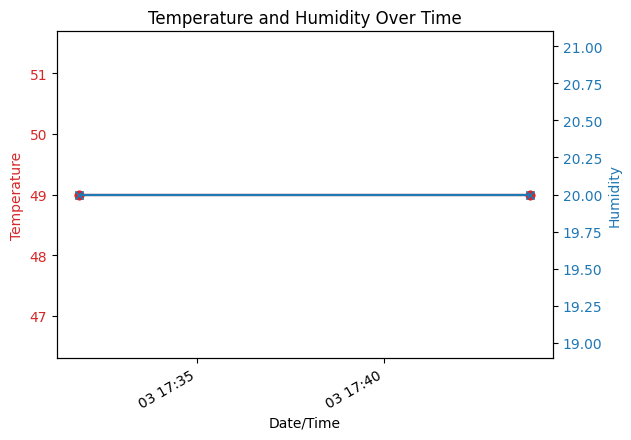
\includegraphics[width=0.5\linewidth]{Images/temp_and_humidity_over_time.png}
    \caption{Temperature and Humidity plotted overtime}
    \label{Temperature and Humidity plotted overtime}
\end{figure} 
last we tested if our code  satisfies our  python code after testing the unit test code we updated see the following message
\begin{figure}[h!]
    \centering
    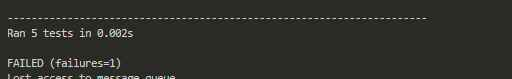
\includegraphics[width=0.5\linewidth]{Images/unit_testoutput.jpg}
    \caption{unit test message for DHT22 module}
    \label{unit test message for DHT22 module}
\end{figure}
\newpage
\subsection{AS312}
\begin{table}[h!]
    \centering
    \begin{tabular}{|c|c|}
        \hline\\
        date/time of record & motion detected(yes/no)\\
        \hline \hline\\
        2024-03-25_15-02-57&False \\
        2024-03-25_15-04-37&True\\
        2024-05-03_18-07-51&False\\
        2024-05-03_18-18-37&True\\
        \hline
    \end{tabular}
    \caption{Recorded data from  AS312 on the \today}
    \label{Recorded data from  AS312 on the \today}
\end{table}
\subsection{DFR0026}
For first test we got  the following table: 
\begin{table}[h!]
    \centering
    \begin{tabular}{|c|c|}
        \hline\\
        Date/time of record & lux values(lux)\\
        \hline \hline\\
        2024-03-25_15-02-57&940\\
        2024-03-25_15-03-13&945\\
        2024-03-25_15-04-37&4963\\
        2024-05-03_18-54-57&1284
        \hline
    \end{tabular}
    \caption{Recorded data from DFR0026 on the 25th of march 2024}
    \label{Recorded data from DFR0026 on the 25th of march 2024}
\end{table}
If this is plotted we get the following:
\begin{figure}[h!]
    \centering
    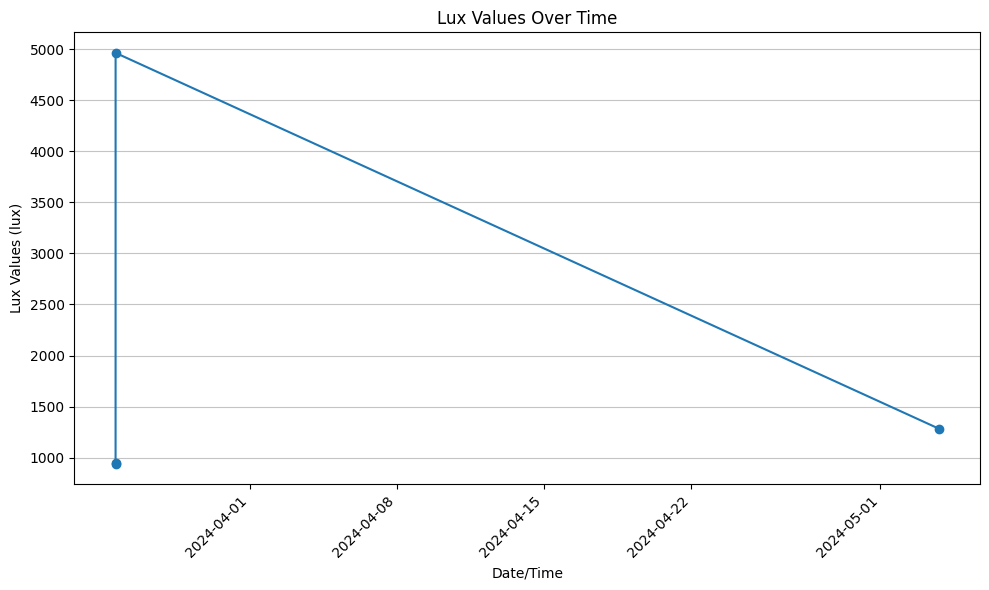
\includegraphics[width=0.5\linewidth]{Images/lux_values_overtime.png}
    \caption{lux values overtime}
    \label{lux values overtime}
\end{figure}
\newpage
\subsection{Raspberry Pi VR 220}
When testing  the Raspberry Pi VR 220 the following picture was taken:
\begin{figure}[h!]
    \centering
    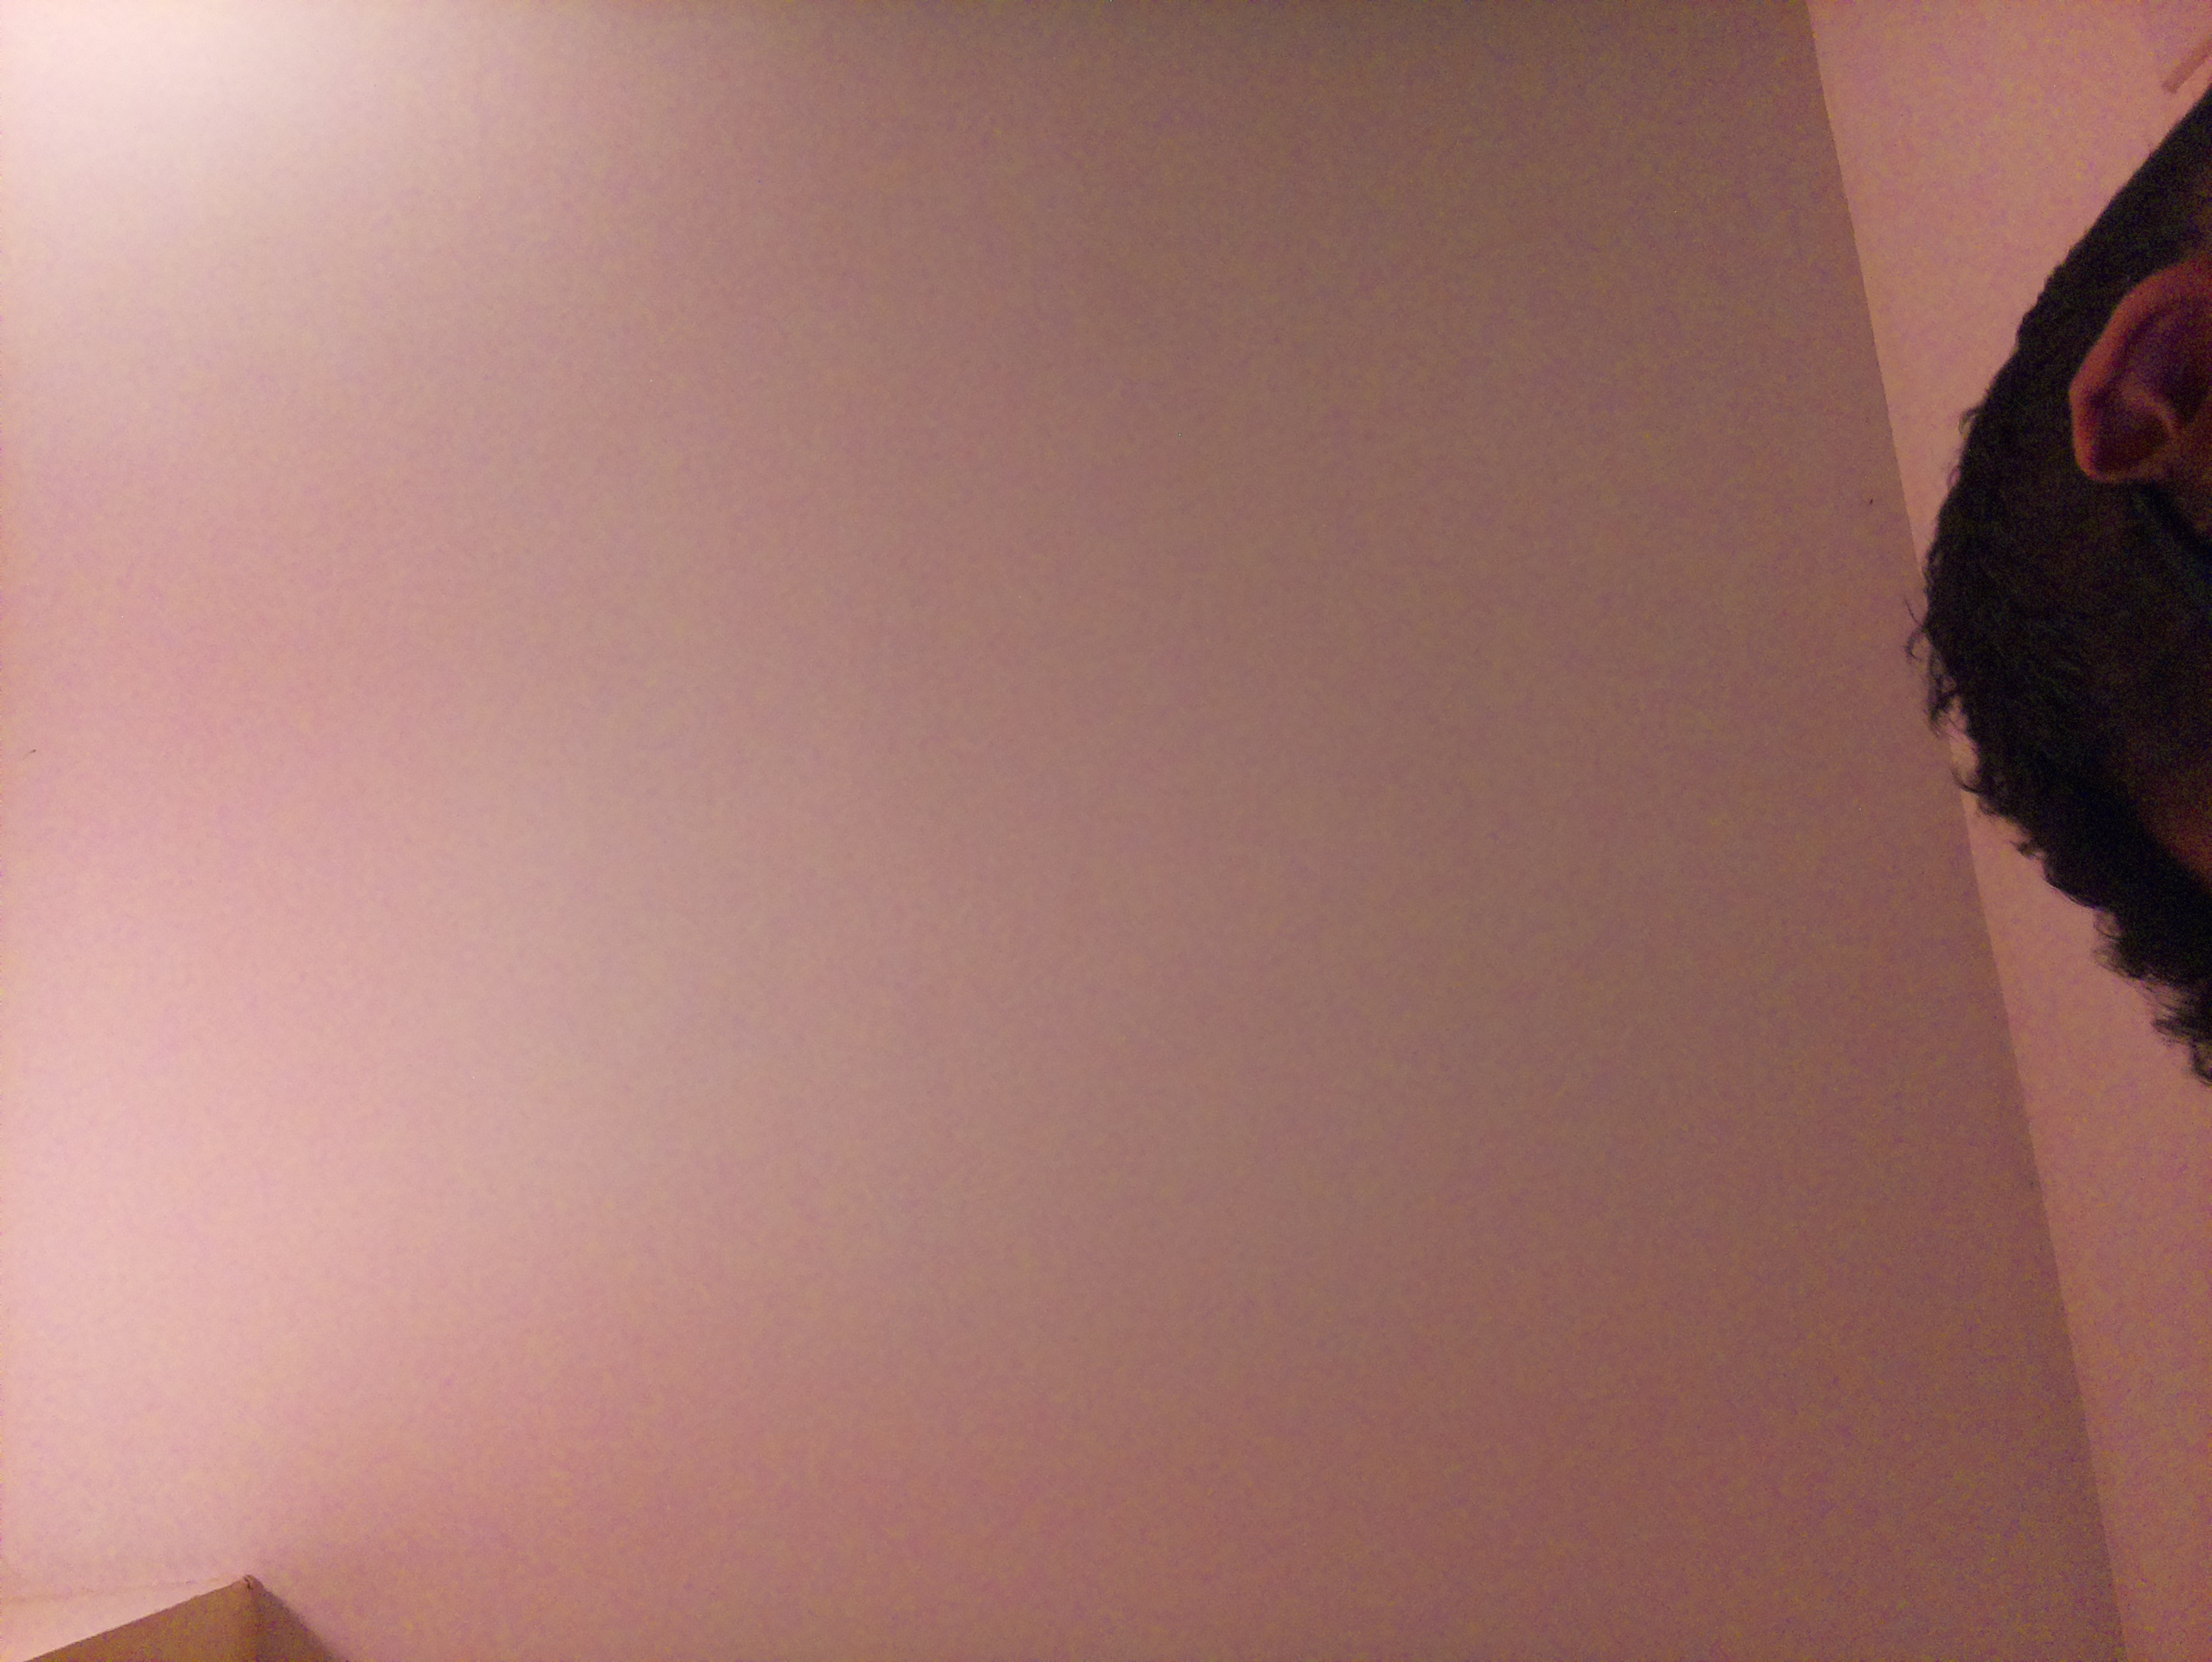
\includegraphics[width=0.4\linewidth]{Images/camera_output_2024-03-21_21-43-16.png}
    \caption{A photo from 25th of march 2024 }
    \label{A photo from 25th of march 2024}
\end{figure}

\section{Recorded data from transceiver}
When testing  the radio module the follow was tested:
\begin{enumerate}
    \item Sending a message across the serial

    \item Sending a txt file across the serial

    \item Sending a csv file across the serial

    \item Sending a image file across the serial

    none results where obtained due to  factor on \pageref{Discussion of Lora module}
\end{enumerate}
 % Include your results content from a separate file

\chapter{Discussion}
\lipsum[1-3]
%In this section we will discuss the following:
\begin{enumerate}
    \item Results of the sensor data
    \item Results of the camera
    \item Results of the Lora module
\end{enumerate}
\section{Discussion of results of Sensor data}
in this section, the data gathered from the sensor will be discussed Note:(\textbf{all tests here were conducted indoors}):
\begin{enumerate}
    \item DHT22 (Temperature \& Humidity):

    On page \pageref{Recorded data from  DHT22 on the 5th of March} compared to the average room temperature which is  20$^o$c, The range of humidity in a room is from 30\% to 60\% in the plot on page \pageref{Temperature and Humidity plotted overtime} note in the file sensor\_data.csv there entries that are 0, this is due to testing different components and make these values as  0. during the development stage of this project we ran unit tests this module as seen on page \pageref{unit test message for DHT22 module}.
    \item AS312 (Motion ):

    As seen on page \pageref{Recorded data from AS312 on the \today} this will output a table that is True when an object is detected and  false when no object is  detected

    \item DFR0026 (Lux ):
    As seen on page \pageref{Recorded data from DFR0026 on the 25th of March 2024} is a table full of lux values according to this \href{https://www.thoughtco.com/lighting-levels-by-room-1206643}{link} we ideally want a lux value of  800 to 1700 lux which satisfies these conditions.
\end{enumerate}
\section{Discussion of Results of camera data}
As seen on page \pageref{A photo from 25th of March 2024} which shows  an image that was taken by the camera  attached to  the pi
\section{Discussion of Lora module}
\label{Discussion of Lora module}
While updating the repository for this section the Pi's SD cards were corrupted due to  a faulty binary file which was  later fixed  but  this error led to the following error message:

\begin{figure}[h!]
    \centering
    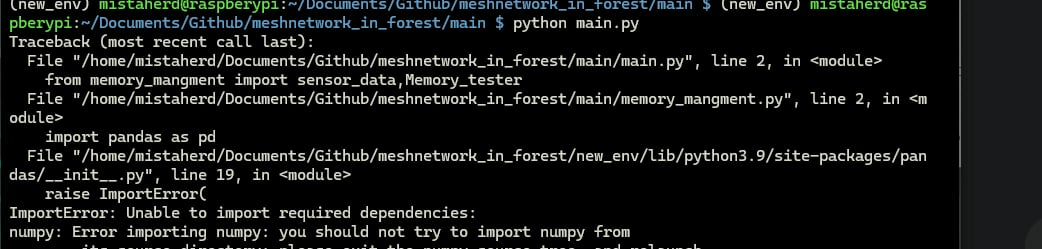
\includegraphics[width=0.5\linewidth]{Images/error_message.jpeg}
    \caption{environment error message}
    \label{environment error message}
\end{figure} % Include your discussion content from a separate file

\chapter{Conclusion \& Future Work }
\lipsum[1-3]
%\section{Conclusion}
\label{ch:conclusion} % For easy referencing
In this final year project, We have explored the implementation and development of mesh networks within the challenging environment of a forest. Through:
\begin{enumerate}
    \item The wireless commutation environment 
    \item The desired characteristics of the sensors
    \item The available electronic devices for this limitation
    \item The limited hardware available
    \item The  fundamental software needed
    \item The Setup of the software
    \item The examination of the programming software needed
    \item The test before the writing of any code 
    \item The discussion of how to record data
    \item The Limitations
\end{enumerate}
\subsection{Key Contributions}

This project has contributed significantly to the understanding of the process of developing mesh networks in forest settings by:

\begin{itemize}
    \item \textbf{Developing a Model:} In this we used serial communication to test the nature of  which the network will send/ receive data from the network 
    \item \textbf{Addressing Challenges:} in a line of sight environment the sending and receiving of images is a hard task due to  how large the file is byte by byte
    \item \textbf{Performance Evaluation:} every method eventually worked via serial but image files had the  most problems
    \item \textbf{Practical Implications:} Schedule the sending  and  receiving  of data we can use this to extract the sensor data
    \item \textbf{Familiarity with different tools:} This project forces the project implementation to use the terminal in Linux, bash, In Linux the concept of Dev files are files where the port can be defined for example port 80 on the window would be \textcolor{yellow}{/dev/tty80}, also the addition of tools like ssh which allowed remote connection to the Pi board, batch files used to make these connections easier, A stronger familiarly with git was gained due to the keeping the project version controlled, A display of further knowledge of python was gain due to  project such as  using virtual environments and  how to properly structure OPP program, An understanding of  TDD for coding projects was gained where the implementor is forced to  use these methods
\end{itemize}
\section{Sources of Error}
In this section, the following will be discussed:
\begin{enumerate}
    \item Radio module
    \item MCP3008
    \item Time management
    \item Lack of knowledge of Linux OS
    \item Camera
    \item Lack of hat for sensors
\end{enumerate}
\subsection{Radio Module}
This section will discuss the problems noticed while working on this:
\begin{enumerate}
    \item When trying to look for radio modules for the MM2 Series 900 MHz this part couldn't be ordered due to the vendor only accepting business customers this cost 4 weeks of research to look for another module
    \item Once the appropriate modules were after looking and noticing that the documentation was very poor it did help as well.
    \item One avenue not expected of this was enabling the serial. So once we enable via sudo raspi-config, and use the code from this \href{https://github.com/sbcshop/Lora-HAT-for-Raspberry-Pi}{link} (use lora\_receiver.py and lora\_transmitter.py) when we get the following error:

    \begin{figure}[h!]
        \centering
        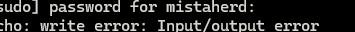
\includegraphics[width=0.5\linewidth]{Images/write_issue_linux_ser.png}
        \caption{Issue when trying to write to serial }
        \label{Issue when trying to write to serial}
    \end{figure}
    This issue took a lot of time to fix a simple chmod rw operation will fix the issue which should be indicated in the documentation but there isn't.
    \item After getting a working demo on all use cases of the module the image file caused the most issues this was due to the nature of how large the large data in an image file further research should have been put into how an image is sent across a communication channel.
    \item The lack of documentation meant time was spent looking at the components on board and finding how they worked. 
\end{enumerate}
\subsection{MCP3008}
In this section the Errors that occurred with this module are the following:
\begin{enumerate}
    \item When it came to ordering this part, There were issues with the venter so another ADC had to be chosen this caused another few weeks to go by.
\end{enumerate}
\subsection{Lack of knowledge of Linux os}
This section will discuss the errors that occurred theses are the following:
\begin{enumerate}
    \item Since the lack of experience with Linux is evident  this led to time spent learning about certain commands that will help with the project concepts such as  piping  commands nmap where  foreign before this project a lot of time was spent learning the best tools for this project
\end{enumerate}
\subsection{Camera}
This Section will discuss the errors that occurred with this module these are the following:
\begin{enumerate}
    \item When using the python file "camera.py" this wouldn't comply due to how the old library is no longer supported this costs around 2 weeks due to finding different forms and tracking the right library down eventually. the decision was made to make a bash command  to run the camera
\end{enumerate}
\subsection{Lack of hat for sensors}
This Section will discuss the issues of this which are  the following:
\begin{enumerate}
    \item When wiring up all the sensors it took several minutes to wire the devices up which led to miss wiring the temp sensor which blew  leading to an order for a replacement to be made
    \item This issue along with the could have led to  the code being simpler in nature them what is present in the repository
\end{enumerate}
\section{Future Work}

While this project hasn't achieved its core objectives, several avenues for future research and development remain open:

\begin{itemize}
    \item \textbf{Sockets:} The project could have ventured into socket programming, A socket is an endpoint of a two-way communication link between two programs running on the network. we picked serial communication for testing but this is where the main server and client can defined.
    \item \textbf{Helpful Tools:}  Linux has a wide range of networking tools such as:
    \begin{itemize}
        \item\textbf{Nmap} is a network scanner designed to discover hosts and services on a computer network. It sends packets and analyzes the responses to gather information 
        \item \textbf{ifconfig} Which provides extensive control over interfaces, addresses and routes
        \item \textbf{traceroute} Traces the route packets take to reach a destination
        \item \textbf{route} Displays or manipulates the kernel's IP routing table
        \item \textbf{arp} Displays and manages the Address Resolution Protocol (ARP) cache, which maps IP addresses to MAC addresses
        \item \textbf{tcpdump} Captures and analyzes network traffic, useful for diagnosing network issues.
        \item \textbf{iftop} Displays a real-time bandwidth monitor for network interfaces.
    \end{itemize} 
    \item \textbf{Energy Efficiency:} Investigate further what can be done to make  our system more energy effective i.e piplineing the sensor data
    \item \textbf{Security:} Investigate how to make our data secure via RSA and different protocols
    \item \textbf{PCB board :} After testing the board one problem was wiring up the sensor a potential for making a custom  Pi hat that will provide an easy way of connecting  our sensor 
 
   
\end{itemize}
\newpage
\subsection{Final Remarks}
The deployment of mesh networks in forest environments holds immense promise. The work provided here doesn't outline how to achieve this but can be viewed as a method to achieving  this nature % Include your conclusion content from a separate file
\addcontentsline{toc}{chapter}{Bibliography}
\bibliographystyle{ieeetr}

\bibliography{References.bib}

\appendix
\chapter{Appendix A}
\FloatBarrier
\chapter{Python Scripts}
\label{appPythonScripts}

\FloatBarrier
\chapter{Bash scripts}
\label{appBashScripts}

\clearpage
\addcontentsline{toc}{chapter}{Index}
\printindex
\end{document}
